\documentclass[../class_mech_main.tex]{subfiles}



\begin{document}

\chapter{Electrodynamics}

\todo{wouldn't it make sense to have this as chapter 3? Or even 2 (because we often study electrical stuff in analytical mechanics)?}



In classical mechanics, particles are mostly assumed to be really simple. They have a mass and move in some way. But some interactions that are observed experimentally cannot be explained by mass. A natural conclusion is that many real particles (and objects) must have additional properties that explain the observations. Ignoring quantum-mechanical effects for now, perhaps the most important of these properties is \Def{charge}, which induces electromagnetic interactions between charged objects.

From Newtonian theory, we expect that the examination should be relatively simple: through experiments, we find an expression for the electromagnetic force, and then examine all phenomena based on that. As \cite{Griffiths_2017} describes in his introduction to Chapter 1, this can be done, but the resulting expression turns out to be extremely complicated. Therefore, it makes sense to instead build up an understanding using a less ad-hoc approach and study the different regimes first, before combining them all in the most general discussion.


One further note concerns the physical realm of electrodynamics. By examining phenomena exhibited by charges, we wander on the verge between classical, Newtonian physics and relativity. We treat as part of classical physics (the scope of this summary) here because it is not necessary to worry about relativistic effects for many applications (though we could \emph{choose} to do so, as we shall see). But the fact that Einstein developed relativity largely to explain electrodynamics properly should tells us that it is an inherent relativistic theory.


As a last comment, this chapter makes heavy use of math discussed in Sec.~\ref{sec:diff_geo}, where the relation of differential and integral laws is explored.



    \section{Electrostatics}
All charges at rest

        \subsection{The Basics}
We will commonly denote charge by $q$. Every charge is a multiple of an \Def{elementary charge} $e$,
\begin{equation}
    \eqbox{
        q = N e
    }, \; N \in \mathbb{N}
    , \quad
    \eqbox{
        e = 1.602 \cdot 10^{-19} \, \unit{\coulomb}
    } \, .
\end{equation}
This is a crucial difference to masses, where no such \enquote{elementary mass} is known.

A (idealized) concept that is frequently used is that of a point/test charge (closely related to point/test mass), which has all of its charge $q$ concentrated in a point of infinitesimal spatial extent. For a collection of point charges $q_i$, we can use that charge is additive (like mass) to obtain the total charge as
\begin{equation}
    \eqbox{
        Q = \sum_i q_i
    } \, .
\end{equation}
Note that test charges are free to move because the force they exert is proportional to their charge and thus practically zero.

While point charges are a powerful concept, and quite flexible too (in the sense that anything looks like a point charge, if viewed from large enough distance), we cannot always avoid looking in detail at how charges are distributed across a spatial region. In the most general case, we can study this using a charge distribution $\rho = \rho(\vec{r}, t)$, representing charge per volume. (While lines and surfaces are strictly speaking also volumes, just in dimensions lower than three, it is common to use $\lambda, \sigma$ for the density on a line, surface, respectively.) The total charge enclosed in a certain volume $\mathcal{V}$ can then be calculated as
\begin{equation}
    \eqbox{
        Q = \int_\mathcal{V} dq = \int_\mathcal{V} \rho \, d\mathcal{V}
    } \, .
\end{equation}
For a point charge with charge $q$ at $\vec{r}_0$, we can write down the distribution
\begin{equation}
    \eqbox{
        \rho(\vec{r}) = q \, \delta(\vec{r} - \vec{r}_0)
    }
\end{equation}
and similarly, for a collection of charges $q_i$,
\begin{equation}
    \eqbox{
        \rho(\vec{r}) = \sum_i q_i \, \delta(\vec{r} - \vec{r}_i)
    } \, .
\end{equation}
Here we port discrete to continuous by adding a $\delta$-function for each charge, which turns integral into sum.\\


-> note that point charge is flexible notion; if distance to $\vec{r}$ is large, then even macroscopic source can be taken as point charge! (another similarity to mass and gravitation)



Although one can make the point that any electric interaction means we leave the realm of Newtonian physics and enter the one relativity, we still study interactions in terms of forces. The electrical \Def{Coulomb force} (also: \Def{Coulomb's law}) from charge 1 onto charge 2 is
\begin{equation}
    \eqbox{
        \vec{F}_C = \vec{F}_{C, 1 \rightarrow 2}
        = \fpeps q_1 q_2 \, \frac{\vec{r}_{12}}{\norm{\vec{r}_{12}}^3}
        = \fpeps q_1 q_2 \, \frac{\vec{r}_2 - \vec{r}_1}{\norm{\vec{r}_2 - \vec{r}_1}^3}
    } \, .
\end{equation}
where $\vec{r}_{12} = \vec{r}_2 - \vec{r}_1$ is the displacement vector connecting object 1 to object 2 (because of this, it naturally obeys the third law). Similarly to Newton's law of gravitation, it has been found empirically. It, too, obeys the superposition principle,\footnote{As \cite{Griffiths_2017} notes in the first footnote of Chapter 2, this is only the case because $\vec{F}_C$ is linear in the charge. This is truly an empirical insight and should be appreciated appropriately.} which means the Coulomb force from a charge distribution $\rho$ onto a test charge with charge $q$ at position $\vec{r}$ is
\begin{equation}
    \eqbox{
        \vec{F}_C(\vec{r}) = \fpeps q \int_{\mathcal{V}'} \rho(\vec{r}') \frac{\vec{r} - \vec{r}'}{\norm{\vec{r} - \vec{r}'}^3} \, d\mathcal{V}'
    } \, .
\end{equation}
$\epsilon_0$ is a constant, the \Def{permittivity of free space} (\cite{Griffiths_2017} does not like this name, but it is what it is) and in SI units, it takes the value
\begin{equation}
    \eqbox{
        \epsilon = 8.854 \cdot 10^{-12} \unit{\coulomb\squared\per\newton\per\meter\squared}
    }
\end{equation}
which means that the factor $\fpeps$ takes a really large value $\sim 10^{12}$ (which may, of course, be cancelled by small charges or large distances to make the total force small).

Another interesting property of charges that we did not have before with masses etc.~is the following: charges can be positive \emph{and negative}. Thus the Coulomb force can be attractive ($q_1 / q_2 < 0 \Rightarrow \vec{F}_{12} \parallel \vec{r}$) and repulsive ($q_1 / q_2 > 0$), one of many effects that this has.


-> interesting observation: let's say we put two test charges together; of course, they would also have some mass usually, so gravitational interaction would also be present -> thing is: $e \sim 10^{-19}$, while $m_e \sim 10^{-31}$ and the constants in front of charge are also much smaller for gravitational interaction! $G \sim 10^{-11}, 1/\epsilon_0 \sim 10^{12}$; means that on short ranges, electromagnetic interaction is by far dominant; only over long ranges, gravitational takes over because there is no negative mass (for Coulomb force, as we integrate over larger region of space, positive and negative forces will almost completely cancel; mass, on the other hand, only accumulates)


-> nice by Griffiths: Coulomb + superposition principle are all we need for electrostatics; to infer laws, we just exploit mathematical consequences of the specific form it has


-> note that the fact that we can write $\rho(\vec{r}) = \sum_i q_i \, \delta(\vec{r} - \vec{r}_i)$ is consequence of superposition principle; because we can take viewpoint that Coulomb only specifies interaction between two individual particles, and that the total force can be written in such a form inherently relies on us being able to add together forces from each charge thanks to the superposition principle



        \subsection{Electric Field}
Coulomb's law is great for determining the mutual forces of charged bodies onto each other. But sometimes we would like to get such a statement about how a body interacts electrically that is independent of the nature of the second body. This is a very tricky question because a second body is required for an effect/interaction to be measurable at all. Thus we have to apply a trick, which consists of introducing \Def[test charge]{test charges} with $q_2 \rightarrow 0$ (similar to the concept of a test mass in mechanics that had $m \rightarrow 0$). The force exerted by this object likewise goes to zero -- but by the third law, so does the force felt by it, which means this is not the measure we seek for the strength. Instead, recognize that, while the force tends to zero, the quotient of force and charge does not. This defines the notion of \Def{electric field} emitted by charge $q$ at position $\vec{r}_0$
\begin{equation}
    \eqbox{
        \vec{E}(\vec{r})
        % = \lim_{q_2 \rightarrow 0} \frac{\vec{F}_C}{q_2}
        = \lim_{q_2 \rightarrow 0} \frac{\vec{F}_{C, \vec{r}_0 \rightarrow \vec{r}}}{q_2}
    } \, ,
\end{equation}
which is our desired measure of how strongly $q$ interacts with its surroundings. (\cite{Griffiths_2017} describes the field as \enquote{force per unit charge}, which is mathematically equivalent to our definition.)


For a collection of charges, described by its distribution, we can always use Coulomb's law to express it more explicitly as
\begin{equation}\label{eq:efield_general}
    \eqbox{
        \vec{E}(\vec{r}) = \fpeps \int_{\mathcal{V}'} \rho(\vec{r}') \frac{\vec{r} - \vec{r}'}{\norm{\vec{r} - \vec{r}'}^3} \, d\mathcal{V}'
    } \, .
\end{equation}
(Important note: careful when carrying out such an integral in practice. Depending on the basis used to write out $\vec{r}, \vec{r}'$, we might have to keep the unit vectors $\unitvec{k}$ in the integrals. For Cartesian coordinates, this is not required, but for curvilinear we cannot avoid this. \cite{Griffiths_2017} therefore advises to always use Cartesian coordinates to calculate electric fields.) In case of a point charge, this yields
\begin{equation}
    \eqbox{
        \vec{E}(\vec{r}) = \fpeps q \frac{\vec{r} - \vec{r}_0}{\norm{\vec{r} - \vec{r}_0}^3}
    } \, .
\end{equation}
-> this particular expression is supremely useful because it is easily integrated in spherical coordinates; using the superposition principle can then, possible, allow us to calculate arbitrary fields more easily (also true if $\rho$ is a function of $r$ only, not direction, or even entirely uniform; then we do not even need to use superposition for this to be true)

-> fields are cool because no matter how charge emitting field is constituted, as soon as we have field, we also get the force on charge $q$ as $\vec{F} = q \vec{E}$ (consequence of superposition principle)


-> but what \emph{is} an electric field truly? This is not so easy to answer, in the end a matter of personal preference of how you think about it. Is certainly a mathematical function that assigns scalar value to each point in space, which measures strength of electric interaction at this point with charge at some fixed position



interesting feature of Coulomb force coming from a charge distribution $\rho$: from entirely mathematical considerations (cf.~Eq.~\eqref{eq:gradient_rnorm}), we can show that it has a \Def{potential} $\varphi$\footnote{Unfortunately, \cite{Griffiths_2017} uses the variable $V$ for our $\varphi$. We do adopt this because $V$ is used for the potential of the Coulomb force below, continuing how things are named in Newtonian physics.} (though this also makes sense physically, Coulomb is a central force, and those always have a potential); this is quantified equivalently by
\begin{equation}
    \eqbox{
        \vec{E} = - \grad \varphi
    }
    \quad \quad
    \eqbox{
        \varphi(\vec{r}_0) - \varphi(\vec{P}) = - \int_{\vec{P}}^{\vec{r}_0} \vec{E}(\vec{r}) \cdot d\vec{r}
    } \, .
\end{equation}
(One quick note: the lower limit $\vec{P}$ just comes out as an integration constant that vanishes when taking a gradient, so it is arbitrary. This is a common theme with potentials, only potential differences are uniquely determined. It is common to choose $\vec{P} = \infty$ because for real-world electric fields, $V(\infty) = 0$. If you have a textbook problem where this is not the case, you are free to choose $\vec{P}$ differently.) The explicit path $\vec{C}$ taken between the integration limits does not influence the result here (a consequence of the fundamental theorem of calculus, due to the existence of the anti-derivative $V$; equivalently, a consequence of $\curl \vec{E} = 0$), so we straight up omitted here and just wrote down the integration limits.


Let us now collect a few notes regarding the potential, especially regarding names in this context:
\begin{itemize}
    \item Careful with the name \enquote{potential}. In mechanics, potentials of forces were directly equal to energy. However, \enquote{potential} is a more general, in fact mathematical term, and we are looking at the potential of a field in case of $\varphi$. It is possible to define an analogous potential for the Coulomb force in
    \begin{equation}
        \eqbox{
            V \coloneqq q \varphi
        } \, ,
    \end{equation}
    and as we will see in Sec.~\ref{subsec:estatics_energy}, this potential is indeed related to the energy of an electrostatic field. But the initial point stands, we have to be more careful with the identification because several notions of potential exist.
    
    (Note that the existence of $V$ implies that the Coulomb force is conservative. We could have seen this immediately since it is a central force.)
    
    
    \item A potential difference $\Delta \varphi$ between two points is called \Def{voltage}. This name is closely connected to the unit of the potential, which is defined as \Def{volt}. Since the expression of $\varphi$ is just force ($\unit{\newton}$) multiplied with $\unit{\meter}$ (due to different power in norm) and divided by $\unit{\coulomb}$ (because we are missing a $q$); thus,
    \begin{equation}
        \eqbox{
            \qty[\varphi] = \unit{\newton \meter \per \coulomb} \unit{\joule \per \coulomb} \eqqcolon \unit{\volt}
        }
    \end{equation}
    (I guess here it would be cool to use $V$ instead of $\varphi$...)


    \item The remarkable fact that all information from a \emph{vector} field (three components/numbers for each point in space) is already contained in a \emph{scalar} field (one number for each point in space) is quickly explained by the fact that the specific form and physical origin $\vec{E}$ do not permit fully independent components (e.g., the curl vanishing is inherently a condition on combinations of components, essentially reducing the degrees of freedom of them)
\end{itemize}


Coulomb force has superposition principle, electric field has it, and due to the linearity of the gradient, the potential also has it. Similarly, the preceding discussions allow us to write down a general expression for $\varphi$. Eq.~\eqref{eq:efield_general} implies
\begin{equation}\label{eq:potential_general}
    \eqbox{
        \varphi(\vec{r}) = \fpeps \int_{\mathcal{V}'} \rho(\vec{r}') \frac{1}{\norm{\vec{r} - \vec{r}'}} \, d\mathcal{V}'
    } \, .
\end{equation}
(Note that the sign in $\norm{\vec{r} - \vec{r}'}$ is important here because it determines the sign in the electric field Eq.~\eqref{eq:efield_general}.)


-> existence of potential implies curve-integrals are path-independent; we define \Def{voltage} based on this, as difference of scalar potentials; is related to work in straightforward manner, via $W = q U$ (is amount of work done on a charge, independent of actual charge that is moved, right? Same relation as between electric field and force) \todo{rather introduce notion of voltage later on?}


-> say we have sphere of radius $R$ with uniform surface charge. What is potential? Gauss's law yields field outside of sphere (the cool trick with symmetry), while inside is zero (because no charge enclosed). So for $r \geq R$, we can obtain $\varphi$ by the usual integration of $E$ from our reference point $\infty$ to $r$. What about $r < R$? Field vanishes inside, does it too? Well, no, since we start our integration from $\infty$ and not zero. But intuition is not completely off, $\rho(\vec{r}) = 0$ for these points, so $\varphi(r > R) = \varphi(R) = \mathrm{const}$ (as it should, field as gradient of potential must vanish)

-> now say we have charge enclosed in sphere of radius $R$



            \paragraph{Field Lines}
convenient tool to visualize vector fields, replace drawing the actual vector with its magnitude in many points in space

-> magnitude of field can now be read off from density of field lines


some rules:

field lines are drawn from positive to negative charges, i.e.~they represent direction of force acting on a particle with positive charge; to make things even more clear, they begin on negative charges and end on positive ones (so electrons move against the field lines in an electric field)

if we start to draw a field line, we must either also draw its ending (though we might leave out some part in between, in case they extend too far out) or they must go to infinity; this must be the case since $\vec{E}$ is divergence-free in free space

be consistent: if charge $q$ has four field lines, then a charge $2q$ in the same plot should get eight lines (this is motivated by Gauss's law, which we learn about in a minute)


another possibility to visualize fields: \Def{equipotential lines}, i.e.~lines where $V = \mathrm{const}$; these are everywhere perpendicular to the field lines



        \subsection{Maxwell Equations}

straightforward question: what is \enquote{total electric field} of some charge distribution $\rho$? For that, integrate over surface $\mathcal{S}(\mathcal{V})$ enclosing volume $\mathcal{V}$ in which $\rho$ is located spatially. We can do that:
\begin{equation}\label{eq:gauss_law_integral}
    \eqbox{
        \oint_{\mathcal{S}(\mathcal{V})} \vec{E} \cdot d\vec{\mathcal{S}} = \frac{Q}{\epsilon_0}
    }
\end{equation}
where $d\mathcal{S}$ is surface element of $\mathcal{S}$, which is formally turned into a vector by multiplying it with the normal vector $\vec{n}_\mathcal{S}$ of the surface.\footnote{The job of the normal vector is to extract the component of $\vec{E}$ that actually flows through the surface (any flux tangential to the surface is not interesting for the intended use of calculating flux through $\mathcal{S}$).} In words: flux of electric field through a surface is proportional to charges inside! In particular, no charges in $\mathcal{V}$ means that net flow of $\vec{E}$ through $\mathcal{S}$ is zero -- independent of its exact shape, just has to be connected, closed


-> this is first Maxwell equation (or rather integral version thereof)

-> very interesting note: any $1/r^2$ force has its own Gauss law because the only thing we rely on is surface $\propto r^2$, which then cancels radius from force (why is this true for surface? Well, we can always choose \enquote{equivalent} surface to integrate over, where all charges are enclosed as well, namely a sphere of a certain radius -> I think this is the reasoning, not 100\% sure)

moreover, Gauss's law (the other one, relating surface integral to volume integral over divergence) can be used to obtain
\begin{equation*}
    \frac{Q}{\epsilon_0} = \frac{1}{\epsilon_0}\int_\mathcal{V} \rho(\vec{r}) \, d\mathcal{V} = \oint_{\mathcal{S}(\mathcal{V})} \vec{E} \cdot d\vec{\mathcal{S}} = \int_\mathcal{V} \div \vec{E} \, d\mathcal{V}
\end{equation*}
which yields the differential version of first Maxwell,
\begin{equation}\label{eq:gauss_law_differential}
    \eqbox{
        \div \vec{E} = \frac{\rho}{\epsilon_0}
    }
\end{equation}
(Notice how this implies $\vec{E}(\vec{r}) = \fpeps \frac{\div \vec{E}(\vec{r}')}{\norm{\vec{r} - \vec{r}'}} \, d\mathcal{V}'$, which is a reflection and consequence of the Helmholtz theorem \ref{thm:helmholtz_thm})


-> differential might be more concise, but integral one is immensely powerful: it yields total charge in a volume, we only have to measure electric field on some closed surface around it; or, if we know (i) the total charge in the volume and (ii) that the electric field is uniform, it is a shortcut to $\vec{E}$, by using the \Def{Gaussian surface} technique: if the volume $\mathcal{V}$ is sufficiently symmetric (\cite{Griffiths_2017} quotes three possibilities that work: sphere, cylinder, plane; basically shapes for which we have nice curvilinear coordinates tailored to them, so that $\vec{E} \parallel \vec{S}_n$) and the charge density indeed uniform, we can indeed place a volume $\mathcal{V}'$ of the same shape (sphere around sphere, etc) around $\mathcal{V}$, but so that $\mathcal{V}'$ is larger than $\mathcal{V}$; we might still apply it if this symmetry is not present though, namely for systems where individual parts have such a symmetry (compute individual fields, use superposition)


second Maxwell equations is more straightforward:
\begin{equation}\label{eq:maxwell_estat_two}
    \eqbox{
        \curl \vec{E} = 0
    }
    \quad \Leftrightarrow \quad
    \eqbox{
        \oint_\mathcal{C} \vec{E} \cdot d\vec{r} = 0
    }
\end{equation}
where $\mathcal{C}$ is a closed curve (as indicated by use of $\oint$ instead of $\int$)

-> proof is relatively simple: calculate line integral along closed loop of field generated by point charge (turns out to be zero), apply Stokes's theorem to conclude vanishing curl for this setup, use superposition principle to conclude this must be true for general charge distribution (works because curl is linear)



        \subsection{Poisson Equation}
In terms of the potential, Maxwell's equations imply that the potential fulfills the \Def{Poisson equation}
\begin{equation}\label{eq:poisson_eq}
    \eqbox{
        \nabla^2 \varphi = - \frac{\rho}{\epsilon_0}
    } \, .
\end{equation}
Yes, it is actually a consequence of \emph{both} Maxwell equations. While this particular form is derived by inserting $\vec{E} = - \grad \varphi$ into the first Maxwell equation, the second one is implicitly used in the fact that we work with a potential, the existence of which is only asserted by the second Maxwell equation.

-> interesting: we cannot write down analytical, general solutions to PDEs; is because is not possible to write things out with finite number of constants


For the positions where no charges are present, Poisson's equation turns into the \Def{Laplace equation}
\begin{equation}\label{eq:laplace_equ}
    \eqbox{
        \nabla^2 \varphi = 0
    } \, .
\end{equation}
Discussing and solving this equation not only solves physical problems in many cases (namely when no charge is located in the volume where we wish to obtain $\varphi$), but also because an inhomogeneous differential equation like the Laplace equation is always solved by a linear combination of a solution to the full, inhomogeneous equation plus a solution to the corresponding homogenous equation (one can always add the latter and the inhomogeneous equation is still fulfilled). In short, we can learn a lot about the solutions of Poisson's equation by studying those to Laplace's.

-> interesting features are (i) each value of solution is average of its neighboring values and (ii) extrema of $V$ must occur at the boundaries of the volume we integrate over, Laplace's equation does not permit local minima/maxima (\cite{Griffiths_2017} says the following about this: \enquote{Laplace's equation picks most featureless function possible, consistent with the boundary conditions} and \enquote{a harmonic function in two dimensions minimizes the surface area spanning the given boundary line}, where harmonic functions are a general name for the solution of Laplace's equation)

-> \emph{very} interesting: the value of $\varphi$ at point $\vec{r}$ is equal to the average value of $V$ over a spherical surface of radius $R$ centered at $\vec{R}$,
\begin{equation}
    V(\vec{r}) = \frac{1}{4\pi R^2} \oint_\mathrm{sphere} V \, d\mathcal{S}
\end{equation}
(for solution of Laplace's equation)



        \paragraph{Why Use It?}
We have started to look at some of the features and difficulties of dealing with the Poisson equation. But we have not justified why it should even be used. Why should we even want to use this partial differential equation of second order? After all, just give me the charge distribution $\rho$ and I can calculate $\varphi$ and $\vec{E}$ using the formulas \eqref{eq:efield_general}, \eqref{eq:potential_general}.

However, these equations are all stated in terms of integrals that are not particularly easy to evaluate. (Well, at least analytically, since it is seldomly the case that geometries of bodies are sufficiently simple to allow us to use some of the tricks we have seen before. Integrating numerically is also not trivial, though. Partly, this is because the geometry of the involved bodies might be hard to parametrize. \todo{this must play a role here, right?}) More importantly, however, the integration only works if we indeed know $\rho$. As it turns out, this is by no means guaranteed and for many applications, we only know the total charge of a body, but have no clue about how this charge is distributed (which is quite reasonable, there might be a lot of motion due to the interaction of charges, until the equilibrium is reached).

Hence we are sometimes forced to solve differential equations instead of doing integration. If we are indeed interested in positions where $\rho(\vec{r}) = 0$, then we are left with the Laplace equation or equivalently the homogenous Maxwell equation. (The crucial difference to the the integrals in Eqs.~\eqref{eq:efield_general}, \eqref{eq:potential_general} is that they require $\rho$ even if we just want the field in positions where $\rho = 0$.) Having to choose between the two is then a matter of making the most economic decision: we can choose a partial differential equation of second order for a scalar field or a partial differential equation of first order for three scalar fields (each component enters in the Maxwell equation). This is why solving the Laplace/Poisson equation is an important task in electrostatics.



-> Fig.~2.35 of \cite{Griffiths_2017} is incredible, shows how we may translate between $\rho, \vec{E}, \varphi$



            \paragraph{Boundary Conditions}
Differential equations must always be supplemented with a set of suitable boundary conditions. A priori, it is not clear which boundary conditions are suitable, in fact it can be quite difficult to specify them (must be restrictive enough that they constrain solutions, but not too restrictive that they prohibit us from finding a solution at all). For the Laplace and Poisson equation in particular, there are a several possible choices, which each come with a theorem proving that the choice makes a \enquote{good} boundary condition (in form of a uniqueness theorem, which means that the condition permit finding a unique solution).


\begin{thm}[First Uniqueness Theorem]\label{thm:uniqueness_poisson_1}
    The solution to Laplace's equation in a volume $\mathcal{V}$ is uniquely determined if the potential is specified on the boundary surface $\mathcal{S} = \partial \mathcal{V}$.

    This implies that the potential, a solution to Poisson's equation, in a volume $\mathcal{V}$ is uniquely determined if the charge density throughout all of $\mathcal{V}$ along with the potential value on all boundaries is specified.
\end{thm}
This is a remarkable statement: if I find any solution for a given boundary condition, then it is \emph{the} solution -- there is no other one.
-> there are uniqueness theorems, which guarantee that if we find solution, it is the only one


What if we do not know charge density? Was one of the motivations to treat Poisson at all... Luckily, there is another theorem for this case. (Note that we have not formally introduced conductors yet... That is what happens when you follow a book, but structure your notes differently, I guess, but for us a conductor can just be any surface with uniform charge density on it at the moment.)

\begin{thm}[Second Uniqueness Theorem]\label{thm:uniqueness_poisson_2}
    In a volume $\mathcal{V}$ surrounded by conductors and containing a specified charge density $\rho$, the electric field is uniquely determined if the total charge of each conductor is given.
\end{thm}
Hence, what we need is the charges on all conducting surfaces around (inside and outside) the volume of interest. (The region as a whole can be bounded by another conductor or else unbounded, whence the outer boundary is at infinity.)


-> these have interesting consequences for electrostatics, even when we do treat it by solving Laplace's equation: if we find solution for electric field that fits boundary conditions, then this is the unique solution to the problem; the way in which we obtain the solution does not matter. This justifies, for example, the method we had used before to determine uniform electric fields for symmetric configurations

-> one application for this is discussed in next subsection, where we show how to circumvent cumbersome solution techniques like the separation of variables that are normally used to solve Laplace's equation (and that also do not work all the time)



        % \subsection{Image Charges}
            \paragraph{Image Charges}
Here we present a general method to solve Poisson equation subject to certain boundary conditions. The idea is best explained by means of an explicit example: take the problem where a charge is placed in front of a conductor (of infinite length). 

-> idea: to get, for example, field of one charge that shall be perpendicular to certain surface, we can place image charge(s) at certain spot so that field lines cross surface in desired manner (mimick boundary conditions)

-> important detail: the image charges we place must be outside of the area where we are interested in the field, just outside (where, e.g., ground of the charged plate or something is)

-> why does it work? Because we have proven uniqueness theorems for the solution (in particular the first one, \ref{thm:uniqueness_poisson_1}), which means even if we find it by guessing, it is the correct one! And even if the setup studied is entirely different, as long as boundary conditions are same

-> can be done in general, though it is not always easy (highly dependent on geometry of the setup)

% -> isn't idea also somewhat borrowed from multipole expansion? Which allows us to describe arbitrary distribution with discrete number of particles; basically same is now done for boundary conditions


-> potential is guaranteed to agree between the setups; but this determines e-field and force, so they agree too. From this we can, e.g., compute force from conductor onto the charge (noting that $\eval{\frac{\vec{r} - \vec{r}'}{\norm{\vec{r} - \vec{r}'}}}_{\vec{r}' = 0} = 0$ because it is zero component-wise; is single application of l'Hospital)

-> BUT: energy is not same; should also make sense, since image charges only apply to region \emph{above} the plate, but energy calculated for point charge takes into account all space, not just above; by symmetry argument, energy in field of conductor plate is half of the result



        \subsection{Energy}
        \label{subsec:estatics_energy}
\todo{move in front of Poisson equation section, in case we deal with energy of image charges. Or make image charges a subsection again and move it between energy, multipole expansion}
In this section, we answer a very simple question: what is the energy of an electric field? (By \enquote{simple} we mean conceptually simple, as we do not know how simple it is to answer.)

In Newtonian physics, energy is the ability to do work. We continue in this vein, starting with a simple example. Suppose some electric field $\vec{E}$ is present. Then we can use the definition of work to require how much of it is required to move a single charge $q$ between two positions $\vec{a}, \vec{b}$:
\begin{equation}\label{eq:work_test_part_1}
    W = \int_{\vec{a}}^{\vec{b}} \vec{F} \cdot d\vec{r} = \int_{\vec{a}}^{\vec{b}} q \vec{E}(\vec{r}) d\vec{r} = - q \qty[\varphi(\vec{b}) - \varphi(\vec{a})] = - \qty[V(\vec{b}) - V(\vec{a})]
    \, .
\end{equation}
% This is not a surprising result, it matches what we are used to from Newtonian physics. It represents the work that somebody (or something) has to do in order to move a point charge $q$ through the electric field $\vec{E}$, which can be positive (force between $q$ and the field is repulsive) or negative (force between $q$ and the field is attractive).
This is not a surprising result, it matches what we are used to from Newtonian physics. It represents the amount of resistance by the Coulomb upon moving a point charge $q$ through the electric field $\vec{E}$. Conversely, somebody (or something) has to do the work $- W$ on the charge for it to be able to move through the electric field (we need a minus sign here because the force exerted must always be exactly opposite the Coulomb force). $W$ can be positive (force between $q$ and the field is repulsive) or negative (force between $q$ and the field is attractive).

To make sure we do not \enquote{miss out} on work that needs to be done against the electric field, it is common to choose $\vec{a} = \infty$. The work required to move a charge $q$ to the position $\vec{r}$ (which replaces $\vec{b}$ now) is then simply
\begin{eqnarray}\label{eq:work_test_part_2}
    \eqbox{
        W \coloneqq W_{\infty \rightarrow \vec{r}} = V(\vec{r}) - V(\infty) = V(\vec{r}) = q \varphi(\vec{r})
    }
\end{eqnarray}
where the second equality assumes we have $\infty$ as our reference point for $\varphi, V$, so that $V(\infty) = 0$. The last equality means electric work is charge multiplied by voltage. (A quick sanity check: the voltage $\varphi$ had unit volts, charge has coulomb. But since volt = joule per coulomb, work indeed comes out as joule, so everything is nice and consistent.)


Just like before, this result for a single point charge can be generalized to other charge distributions. We do just that now, calculating how much work is required to assemble a certain collection of charges from $\infty$. For the first particle, there is no electric field to do work against, so $W_{\infty \rightarrow 1} = 0$); for the second particle, one has to do work against $\vec{E}_1$; for the third one, against $\vec{E}_1 + \vec{E}_2$; etc. Using the superposition principle for the scalar potential, we end up with
\begin{equation}\label{eq:work_discr_distr}
    W
    = \sum_i W_{\infty \rightarrow i}
    = \sum_i q_i \sum_{j < i} \varphi_j(\vec{r}_i)
    = \frac{1}{2} \sum_{\underset{i \neq j}{i, j}} q_j \varphi_i(\vec{r}_j)
    = \frac{1}{2} \sum_j q_j \varphi_{\qty{q_i}_{i \neq j}}(\vec{r}_j)
\end{equation}
where the weird subscript of $\varphi$ is used to denote the potential of all charges, except for the $j$-th one. We were able to obtain this result because we replaced the sum over $j < i$ with two sums of this kind (accounting for this the factor $\frac{1}{2}$) because it is easier to evaluate. (Note that this expression, as all before, encapsulate only interaction energy, not self energy.)

\todo{this does not account for energy needed to keep the distribution together, right? So I guess we assume that all particles are brought in instantaneously, immediately one after the other. But then I wonder how this is a good model of true energy density...}

in the continuum limit, this reads
\begin{equation}\label{eq:work_cont_distr_1}
    \eqbox{
        W = \frac{1}{2} \int_{\mathcal{V}} \rho(\vec{r}) \varphi(\vec{r}) d\mathcal{V}
    } \, .
\end{equation}
In contrast to Eq.~\eqref{eq:work_discr_distr}, self-energy is now included because we integrate over \emph{all} of $\varphi$ and not just $\varphi_{\qty{q_i}_{i \neq j}}$. By choosing to integrate not only over $\mathcal{V}$, but over all space, this takes the form
\begin{equation}\label{eq:work_cont_distr_2}
    \eqbox{
        W = \frac{\epsilon_0}{2} \int \norm*{\vec{E}}^2 \, d\mathcal{V} \eqqcolon \int w(\vec{r}) \, d\mathcal{V}
    }
\end{equation}
with the energy density $w$ (of electrostatics).


Discussion: Eq.~\eqref{eq:work_test_part_2} does not contain self-energy, while Eq.~\eqref{eq:work_cont_distr_2} does. Therefore, the former is energy we gain when disassembling the charge configuration, but the latter is not.

-> there is good and bad to both: good for first expression is that we do not create charges in practice, we just use already existing electrons etc., so not including self-energy is the correct thing; good for second expression is that it is more complete as it truly contains the total energy stored in the charge distribution (which is nicer if we actually want energy of it, not work needed to assemble)

-> general issue: energy of point charge is (just use Eq.~\eqref{eq:work_cont_distr_2} with single $\delta$-function for $\rho$) infinite. This is not because formula is at fault, but because the concept is weird. Actually, that makes matters worse, though, because point charges are an integral concept in electrodynamics, so the fact that their energy diverges is concerning.

-> very interesting question: where exactly is the energy we have just calculated stored? In the charges? Or is it spread throughout the volume? Well, right now both interpretations are totally valid. We will see later on, though, that it is more customary to think about it as being stored in the field, as a density $w$ throughout all space (this is the preferred interpretation for radiation theory and also general relativity)

-> just like kinetic energy is not additive although velocities are, the electric energy does not obey superposition principle although force/field/potential do (is quadratic in field after all)



        \subsection{Multipole Expansion}
Multipole expansions are a frequently used tool in electrodynamics. The basic idea is to simplify terms of the kind $\frac{1}{\norm{\vec{r} - \vec{a}}}$ by using the general result
\begin{equation}\label{eq:multipole_exp_general}
    \eqbox{
        \frac{1}{\norm{\vec{r} - \vec{a}}}
        % \simeq \frac{1}{r \norm{\vec{e}_r - \frac{a}{r} \vec{e}_a}}
        \simeq \frac{1}{r} + \frac{\vec{r} \cdot \vec{a}}{r^3} + \frac{3 (\vec{r} \cdot \vec{a})^2 - r^2 a^2}{2 r^5}
    } \, .
\end{equation}
(For the explicit calculation, see Eq.~\eqref{eq:multipole_exp_general_calc}.)


-> for large enough distances, we can replace with first/second order to really good approximation! Especially useful to calculate field generated by some distribution, this way we can avoid the really nasty integrals, e.g., for potentials and fields!


Is useful because it allows analysis of arbitrary potential in far-field limit $\norm{\vec{r}} \gg R$, where $R$ is the radius of a ball we assume that the charge distribution can be enclosed in. If this is warranted, so is the expansion
\begin{align}
    \eqbox{
        \varphi(\vec{r})
    }
    &\simeq \fpeps \int_\mathcal{V} \rho(\vec{a}) \qty[\frac{1}{r} + \frac{\vec{r} \cdot \vec{a}}{r^3} + \frac{3 (\vec{r} \cdot \vec{a})^2 - r^2 a^2}{2 r^5}] d^3a
    \\
    &= 
    \eqbox{
        \fpeps \qty[\frac{Q(\mathcal{V})}{r} + \frac{\vec{r} \cdot \vec{p}}{r^3} + \frac{1}{2} \sum_{i, j} \frac{Q_{ij}}{r^5} \vec{r}_i \vec{r}_j]
    }
\end{align}
where for instance
\begin{equation}
    \eqbox{
        \vec{p} = \int_\mathcal{V} \rho(\vec{a}) \vec{a} \, d^3a
    } \, ,
\end{equation}
which is independent of $\vec{r}$. For the rest of this subsection, our goal is to give a physical meaning to each order of the expansion, and also find expressions for the unknown factors. The general idea will be to find a setup that eliminates terms from all order below the one we wish to investigate. This will allow to investigate each order separately.



            \paragraph{Monopole}
Easiest description: $\mathcal{V}$ is so small that it appears as point with no spatial extent. In that case, it can be treated as point charge with charge $Q(\mathcal{V})$. This is the easiest, most simplified description that one can think of, so it naturally corresponds to leading order term
\begin{equation}
    \eqbox{
        \varphi_\mathrm{mono}(\vec{r}) = \fpeps \frac{Q(\mathcal{V})}{\norm{\vec{r}}}
    } \, .
\end{equation}



\begin{figure}
    \centering

    \subfloat[Positive charge]{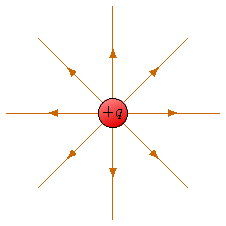
\includegraphics[page=1, width=0.25\textwidth]{pictures/monopole.pdf}}%
    \hspace*{0.1\textwidth}%
    \subfloat[Negative charge]{\includegraphics[page=2, width=0.25\textwidth]{pictures/monopole.pdf}}

    \caption{Monopoles emitted by oppositely charged particles. Taken from \url{https://tikz.net/electric_fieldlines1/}.}
    \label{fig:monopoles}
\end{figure}



            \paragraph{Dipole}
In order to eliminate the monopole term, we need $Q(\mathcal{V}) = 0$. The simplest way to achieve this is to place to point charges with opposite charge together. Placing particle 1 (charge $-q$) in the origin and particle 2 (charge $q$) at a position $\vec{a}$,\footnote{Note that it does not matter whether $q > 0$ or $q < 0$. It is just important that the particles have opposite charge.} the field of this setup is just the superposition
\begin{equation}\label{eq:el_dipole_potential}
    \eqbox{
        \varphi_\mathrm{dip}(\vec{r})
    }
    = \fpeps \qty[\frac{-q}{\norm{\vec{r}}} + \frac{q}{\norm{\vec{r} - \vec{a}}}]
    \eqbox{
        \simeq \fpeps \frac{\vec{r} \cdot \vec{p}}{x^3}
    }
\end{equation}
where we defined the \Def{dipole moment}
\begin{equation}
    \eqbox{
        \vec{p} \coloneqq q \vec{a}
    } \, .
\end{equation}
Not only does this approximated expression look like the second term in Eq.~\eqref{eq:multipole_exp_general}, it \emph{is} this expression for the physical setup of two oppositely charged point masses:
\begin{equation}
    \eqbox{
        \rho(\vec{r}) = q \delta(\vec{r} - \vec{a}/2) - q \delta(\vec{r} + \vec{a}/2)
    } \, .
\end{equation}
Therefore, the second term in Eq.~\eqref{eq:multipole_exp_general} does indeed represent the potential emitted by a dipole, if viewed from far ($r \ll a$).


-> interesting in Griffiths 3.4.3: if total charge is zero, then the dipole moment is independent of the choice of origin


-> in multipole expansion, we have carried out far-field limit, so to understand connection to different order terms better we should do same now for dipole potential; this is what happens in second equality (along with $\lim_{a \rightarrow 0, q \rightarrow \infty}$ so that product remains well-defined) -> this would be the ideal/pure dipole

-> it is not always clear whether the actual dipole with most general field or the second, approximate formula is meant, but we do our best to distinguish the two (\cite{Griffiths_2017} calls these two physical dipole, referring to the full potential with $Q(\mathcal{V}) = 0$ where highest order is dipole term, and ideal/pure dipole, referring to equations where we actually add positive and negative charge -> ahhh no, that's wrong; for some reason, he calls pure dipole the term that comes out of approximation and physical dipole the one comprised of two charges; I do not like this and will not adopt)

-> means I can do two things to improve approximation: increase $r = \norm{\vec{r}}$ or decrease $a$ (we want/need $r \ll a$)


-> field generated by pure dipole can simply be calculated as
\begin{align}\label{eq:el_dipole_field}
    \eqbox{\vec{E}_\mathrm{dip}(\vec{r})} &= - \grad \varphi_\dip(\vec{r})
    % = - \fpeps \qty[-q \frac{-\vec{r}}{r^3} + q \frac{-(\vec{r} - \vec{a})}{\norm{\vec{r} - \vec{a}}^3}]
    \\
    &\eqbox{\simeq \fpeps q \qty[\frac{3(\vec{p} \cdot \vec{r}) \vec{r}}{r^5} - \frac{\vec{p}}{r^3}]}
\end{align}
where we have used potential from Eq.~\eqref{eq:el_dipole_potential}. (Note that the result is linear in $\vec{p}$; since the gradient $\grad_{\vec{r}}$ is also linear, that means it does not matter if we first rewrite $V$ under the assumption $r \ll a$ and the take gradient or first take the gradient to the full potential and then use the assumption $r \ll a$ on the result.)


\todo{write down in spherical coordinates, also insightful}



We have mainly studied the potential and field associated with, i.e.~exerted by, a dipole until now. (From this, one can obtain the force exerted by the dipole by using that the Coulomb force is conservative, $\vec{F}_\mathrm{dip} = q \vec{E}_\mathrm{dip} = - q \grad \varphi_\mathrm{dip}$.) But what about its interaction with another electric field $\vec{E}(\vec{r})$, how does the dipole react to that? From the most general expression, one can quickly obtain the force on the dipole in the dipole approximation:
\begin{equation}\label{eq:dipole_force}
    \eqbox{
        \vec{F}(\vec{r})
    }
    = - q \vec{E}(\vec{r}) + q \vec{E}(\vec{r} + \vec{a})
    \simeq - q \vec{E}(\vec{r}) + q \qty(\vec{E}(\vec{r}) + (\grad \vec{E}(\vec{r})) \cdot \vec{a}
    % If we had chosen \pm d/2 as locations, then we would have to expand around -d/2; but subtracting -d/2 in Taylor-expansion from location at d/2 yields same term
    \eqbox{
        = \vec{p} (\div \vec{E}(\vec{r}))
    }
    \underset{\div \vec{p} = 0}{=} \grad (\vec{p} \cdot \vec{E}(r))
    % \eqqcolon - \grad V(\vec{r})
    \, .
\end{equation}
First of all, that means the dipole force has a potential $\vec{p} \cdot \vec{E}(r)$, i.e.~is conservative. Moreover, in a spatially homogenous field, there is no force acting on a dipole. Nonetheless, there is an effect of the force, namely a torque\footnote{This torque is measured about the center of the dipole, though the first term vanishes trivially for the chosen setup with $\vec{r}_1 = 0$. For more general reference points, the torque becomes $\vec{p} \cross \vec{E} + \vec{r} \cross \vec{F}$.}
\begin{equation}\label{eq:dipole_torque}
    \eqbox{
        \vec{M}
    }
        = \vec{r}_1 \cross \vec{F}_1 + \vec{r}_2 \cross \vec{F}_2
        = \vec{a} \cross q \vec{E}(\vec{r} + \vec{a})
    \eqbox{
        = \vec{p} \cross \vec{E}(\vec{r})
    }
\end{equation}
acting on a dipole, which leads to change in orientation until $\vec{p} \parallel \vec{E}$ where the potential is minimized.\footnote{While an antiparallel configuration formally also extremizes the potential, this configuration corresponds to a maximum, which means it is not stable.} This can be understood similar to a statement in terms of center of mass: the dipole itself is not moving in the electric field, but it constituents do; via the complex interplay of both forces moving in the external $\vec{E}$-field while the two particles still interact, the total effect is merely a rotation of the dipole.



\begin{figure}
    \centering

    \subfloat[Near field]{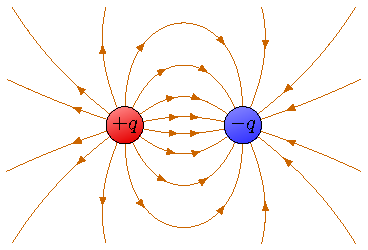
\includegraphics[page=1, width=0.4\textwidth]{pictures/dipole.pdf}}%
    \hspace*{0.2\textwidth}%
    \subfloat[Far field]{\includegraphics[page=2, height=0.3\textheight]{pictures/dipole.pdf}}

    \caption{Dipole in near- and far-field. As we see, the far-field case has a much simpler structure compared to the near-field case, where field lines come in many different forms and shapes. Adapted from \url{https://tikz.net/electric_fieldlines2/}.}
    \label{fig:dipoles}
\end{figure}



            \paragraph{Quadrupole}
now we put two dipoles together in opposite orientation, to eliminate dipole moment. next leading order is thus a \Def{quadrupole}



        \subsection{Boundary Conditions}
% We have seen that boundary conditions play an important part in obtaining the electric field (and thereby interaction between charges) during our discussions of the Poisson equation. Normally, boundary conditions are specified as part of the problem, i.e.~they are given to us by the physical setup. But they cannot be arbitrary, as we can see by thinking in general about the behavior of static electric fields at a boundary surface with surface charge $\sigma$. Our tool to study this has, not surprisingly, been developed by Gauss and is called a \Def{Gaussian pillow} (Fig.~\ref{fig:gaussian_pillow}).

We have seen that boundary conditions play an important part in obtaining the electric field (and thereby interaction between charges) during our discussions of the Poisson equation. Therefore, let us think about them in a little more detail. More specifically, let us examine the behavior of static electric fields at a boundary surface with surface charge $\sigma$ (no matter how $\sigma$ was created or what the exact material properties of the surface are). Our tool to study this has, not surprisingly, been developed by Gauss and is called a \Def{Gaussian pillow} (Fig.~\ref{fig:gaussian_pillow}).



\begin{figure}
    \centering

    \subfloat{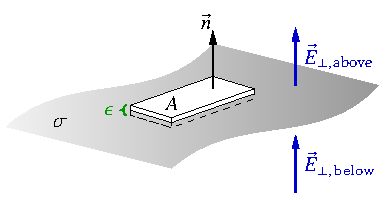
\includegraphics[width=0.45\textwidth,page=1]{pictures/gauss_pillow.pdf}}%
    \hspace*{0.1\textwidth}%
    \subfloat{\includegraphics[width=0.45\textwidth,page=2]{pictures/gauss_pillow.pdf}}

    \caption{Heavily inspired by Figs.~2.36, 2.37 in \cite{Griffiths_2017}. Note that $\vec{E}_{\perp, \parallel}$ are meant to be the fields in the immediate (in fact, infinitesimal) vicinity of the surface.}
    \label{fig:gaussian_pillow}
\end{figure}




-> we enclose very small volume $\mathcal{V} = A \epsilon$, in fact we are interested in $\epsilon \rightarrow 0$ (and, depending on the shape of the surface and how quickly the field $\vec{E}$ varies with position, we might also have to look at $A \rightarrow 0$)

-> idea: evaluate same expression twice, once explicitly and once using Gauss's law

-> second one yields $\int_{\mathcal{S} = \partial \mathcal{V}} \vec{E} \cdot d\vec{\mathcal{S}} = \frac{Q(\mathcal{V})}{\epsilon_0} = \frac{A \sigma}{\epsilon_0}$

-> for explicit evaluation let's look at contributions more closely (we can divide surface and add up integrals): top and bottom each give contribution of the kind $\int_A \vec{E} \cdot d\vec{A} = E_\perp A$ where $E_\perp$ is the field above and below the surface, respectively (which is parallel to the normal vector of $A$ and, if we choose $A$ sufficiently small, constant over it, this is how result comes to be); but when we evaluate the expression for every other area is proportional to $\epsilon$, so the contribution vanishes; accounting properly for orientations of the surfaces (given by their normal vectors), we are left with
\begin{equation}\label{eq:bound_cond_estat_vacuum_1}
    \eqbox{
        E_{\perp, \mathrm{above}} - E_{\perp, \mathrm{below}} = \frac{\sigma}{\epsilon_0}
    } \, .
\end{equation}
(which is also valid in the limit $A \rightarrow 0$ because the $A$'s on both sides cancel.) The electric field is discontinuous when it goes through a surface that has surface charge $\sigma \neq 0$. The latter is the most important part here, though, in case of a uniformly charged sphere for instance the field is actually continuous.


-> selecting any of the surfaces on side of the pillow, we can also calculate the line integral along their boundary $\mathcal{C}$ (e.g., the red line in Fig.~\ref{fig:gaussian_pillow}):
\begin{equation*}
    \int_{\mathcal{C} = \partial \mathcal{S}} \vec{E} \cdot d\vec{r} = E_{\parallel, \text{above}} l - E_{\parallel, \text{below}} l - E_{\perp, \text{above}, \text{left}} \frac{\epsilon}{2} - E_{\perp, \text{below}, \text{left}} \frac{\epsilon}{2} + E_{\perp, \text{above}, \text{right}} \frac{\epsilon}{2} + E_{\perp, \text{below}, \text{right}} \frac{\epsilon}{2}
\end{equation*}
where $l$ is the length of one of the edges of the pillow (the one indicated in Fig.~\ref{fig:gaussian_pillow}). In the limit $\epsilon \rightarrow 0$, many terms do not survive. Further, we must recognize that the integral along a boundary $\partial \mathcal{S}$ is a closed integral by definition -- but then it must be zero, according to the second Maxwell equation (cf.~Eq.~\eqref{eq:maxwell_estat_two}). Therefore, the tangential components fulfil
\begin{equation}\label{eq:bound_cond_estat_vacuum_2}
    \eqbox{
        E_{\parallel, \text{above}} = E_{\parallel, \text{below}}
    }
\end{equation}

Using $\vec{E} = \vec{E}_\perp + \vec{E}_\parallel$ the two conditions on $\vec{E}$ can be summarized in a single, concise equation:
\begin{equation}\label{eq:bound_cond_estat_vacuum}
    \eqbox{
        \vec{E}_\text{above} - \vec{E}_\text{below} = \frac{\sigma}{\epsilon_0} \vec{n}
    } \, .
\end{equation}
(Reminder: $\vec{n}$ is the unit normal vector to the surface.) Please note that this does not mean the field produced by the surface is $\frac{\sigma}{\epsilon_0} \vec{n}$. It might, however, be possible to calculate the surface density and field from the above condition (as shown, e.g., for conductors in the next subsection; cf.~Eq.~\eqref{eq:extfield_surfacecharge_surfacefield}).


In terms of potential, these equations read (note the different sign on the right side)
\begin{equation}
    \grad \varphi_\text{above} - \grad \varphi_\text{below} = - \frac{\sigma}{\epsilon_0} \vec{n}
\end{equation}
or, defining the \Def{normal derivative}
\begin{equation}
    \eqbox{
        \pdv{\varphi}{n} \coloneqq \vec{n} \cdot \grad \varphi
    } \, ,
\end{equation}
they take the form
\begin{equation}
    \eqbox{
        \pdv{\varphi_\text{above}}{n} - \pdv{\varphi_\text{below}}{n} = - \frac{\sigma}{\epsilon_0}
    } \, .
\end{equation}


But while the gradient of the potential inherits a discontinuity from the field, the potential itself \emph{is} continuous since
\begin{equation}
    \varphi_\text{above} - \varphi_\text{below} = \int_{-\epsilon/2}^{\epsilon/2} \vec{E} \cdot d\vec{r} \underset{\epsilon \rightarrow 0}{=} 0
    \quad \Leftrightarrow \quad
    \eqbox{
        \varphi_\text{above} = \varphi_\text{below}
    } \, .
\end{equation}
(We omit integration over the other spatial dimensions here since only the one in the direction normal to the surface matters.)



        \subsection{Conductors}
Until now, all theory we treated happened in vacuum, i.e.~no charges were present outside the ones described by $\rho$. Next, we turn our attention to electric fields in matter. We can divide matter into three different categories, when it comes to their properties regarding charges and interactions with electric fields: \Def[insulator]{insulators} with no free charges, \Def[conductor]{conductors} with one or more free electrons per atom, and \Def[dielectricum]{dielectrics} which are somewhere in between. Insulators do not react in any significant way to external electric field, so discussing them here is kind of pointless. Dielectrics are interesting and we dedicate the next subsection to them. This one is focussing on conductors.


% -> idea of what changes in a medium: total electric field now comes from free charges in $\rho$ \emph{and} from charges in the medium; we assume no free charges in medium for now, but still a total charge can be induced via the formation of small dipoles in the medium -> we look at the macroscopic effect only, i.e.~polarization $\vec{\mathbb{P}}$\footnote{We do not call the polarization $\vec{P}$ because this is already reserved for momentum.}


As we already said, conductors have free charges inside of them, i.e.~electrons attached to atoms that are basically free to roam around in the material. If the number of free charges was infinity, we would call the material a \Def{perfect conductor}. While this is of course not possible in reality, many materials (especially metals) come very close to that and such an approximation is justified. (This is not so different from using a continuous charge distribution $\rho$. In reality, there is always a finite number of particles occupying discrete positions in space, but using $\rho$ can still be more convenient and thus justified.)

Let us now note down some properties, which immediately follow from this definition.
\begin{enumerate}[(i)]
    \item First implication: the net field inside the conductor must be zero. This is because an external field exerts a force on the free electrons, which are pushed opposite to the field lines. In the process, the electrons (and holes, i.e.~positive charges, they leave behind) form a field of opposite direction, the \Def{induced field} formed by the \Def{induced charges}. This process ends once there is no force on the free charges anymore, i.e.~equilibrium is only reached when $\vec{E}_\text{int} = - \vec{E}_\text{ext} \quad \Leftrightarrow \quad \vec{E}_\text{int} + \vec{E}_\text{ext} \eqqcolon \vec{E}_\text{total} = 0$. This flux happens really fast, practically instantaneously for most purposes (so we do not have to argue so much about how we are still in electro\emph{statics}).
    
    (Important: this does not mean the field in all space is zero. The field coming from the free charges outside of the conductor can look very different than the field inside. \todo{put in figure?})


    \item Direct implication from (ii): $\frac{\rho}{\epsilon_0} \div \vec{E}_\text{total} = 0$, there is no net charge inside the conductor. This does \emph{not} mean there are not free charges at all; there are free electrons, but they are bound to the atoms and their charges cancel.
    

    \item Charges must reside on the surface. As \cite{Griffiths_2017} says, \enquote{That's the only place left}. But it also makes sense from what we noted about the motion of electrons in the external electric field.
    
    (A very interesting note on this is that such a behavior only occurs in 3D, lower-dimensional materials are very different. \cite{Griffiths_2017} further points out on page 99 that this is inherently related to the $\flatfrac{1}{r^2}$-nature of the Coulomb force.)

    
    \item A conductor is an equipotential. This is clear since the potential is related to an integral over the electric field, but $\vec{E}_\text{total} = 0$. We can also conclude it from $\vec{E} = - \grad \varphi = 0$, take your choosing.
    
    
    \item $\vec{E}_\text{total}$ is perpendicular to the (outer) surface of the conductor. The argument is simple, if there were any tangential component, then this would exert a force on the free electrons in the conductor and there would immediately be flux of electrons until this tangential component is cancelled.
\end{enumerate}


-> charges spread out as much as possible still (because they repel each other), but all of them (again, \enquote{all} means net charge) reside on the surface; a viewpoint confirming this is energy: all charges on surface is configuration of the system with minimal energy


\begin{ex}[Cavities In Conductors]
    Here is a fun thought experiment: what happens if we carve a hole (cavity) into of a conductor? Does it contain a field? Does the answer to this depend on whether the cavity itself contains charge?

    First of all, if a charge $q$ is present in this cavity, then the field inside will not be zero. -> charges exert field, which induce charge on wall where cavity, conductor intersect as well (and opposite of this charge is induced on outer conductor wall)

    \todo{I do not understand this fully, at least not how this is supposed to work when external field is present; example with no external field makes sense, though (where cavity produces net field equal to the one inside, because it is communicated outside via influence)}

    Griffiths Figs.~2.44, 2.45 are nice

    % \\

    How about the case where no charge is in the cavity? In that case, $\vec{E}_\text{total} = 0$ from inside the conductor must translate to the inside of the cavity as well. We can see this by asking the simple question: where would the any field line beginning in the cavity begin and end? Since field lines start and end on charges, none of which are present in the cavity, the only possibility is that the line starts and end on the cavity wall. So far, there is nothing unreasonable, such a field between two points on the cavity could exist. But if we close the field line with a path that goes through the conductor, where $\vec{E} = 0$, then $\oint \vec{E} \cdot d\vec{r} \overset{!}{=} 0$ requires that the field we picked up when going through the cavity must also be zero.

    Griffiths Fig.2.47 is nice visualization of this

    In other words, if you surround yourself with a conducting surface (which need not be entirely closed), you are safe against any electric field from the outside. This construction is called a \Def{Faraday cage} and is the reason why lightning strikes have no effect on people in cars or planes.
    \todo{we need the cage to be grounded}
\end{ex}



            \paragraph{Field Of And Force On A Conductor}
One of the properties of a conductor is that the field inside of it is zero, $\vec{E}_\text{below} = 0$. The boundary condition Eq.~\eqref{eq:bound_cond_estat_vacuum} we have derived earlier\footnote{We did not assume the surface to be a conductor during the derivation, but the answer still applies if the surface charge was induced on a conductor.} then implies that the field just outside the conductor is given by
\begin{equation}\label{eq:conductor_field_above}
    \eqbox{
        \vec{E}_\text{above} = \frac{\sigma}{\epsilon_0} \vec{n}
    } \, .
\end{equation}
Combining $\vec{E}_\text{surface, below} + \vec{E}_\text{ext, below} = \vec{E}_\text{below} = 0$ on the inside together with $\vec{E}_\text{surface, below} = - \vec{E}_\text{surface, above}$ and $\vec{E}_\text{ext, below} = \vec{E}_\text{ext, above} \eqqcolon \vec{E}_\text{ext}$ (since the external field does not change direction) yields
\begin{align*}
    \vec{E}_\text{above}
    = \vec{E}_\text{ext, above} + \vec{E}_\text{surface, above}
    = \vec{E}_\text{ext, above} - \vec{E}_\text{surface, below}
    = \vec{E}_\text{ext, above} + \vec{E}_\text{ext, below}
    = 2 \vec{E}_\text{ext}
\end{align*}
and thus (Eq.~\eqref{eq:conductor_field_above}, which follows from Eq.~\eqref{eq:bound_cond_estat_vacuum})
\begin{equation}\label{eq:extfield_surfacecharge_surfacefield}
    \eqbox{
        \vec{E}_\text{ext} = \frac{1}{2} \vec{E}_\text{above} = \frac{\sigma}{2 \epsilon_0} \vec{n}
        = \vec{E}_\text{surface, above} = - \vec{E}_\text{surface, below}
    } \, .
\end{equation}
Given the external field that we as experimentalists apply, this determines the surface charge that accumulates on the conductor (and thus the field produced by the conductor surface).


Now, say the total charge on the surface is $Q = \int \sigma \, d\mathcal{S}$. The total force on the surface exerted by $\vec{E}$ is $\vec{F} = Q \vec{E}$, which means we can define a force per unit area
\begin{equation}
    \vec{f} = \sigma \vec{E} \, .
\end{equation}
There exists an ambiguity which field should be used here, $\vec{E}_\text{below}$ or $\vec{E}_\text{above}$? It turns out that their average is what we should take, i.e.
\begin{equation}\label{eq:estat_force_per_area}
    \eqbox{
        \vec{f} = \sigma \frac{1}{2} (\vec{E}_\text{below} + \vec{E}_\text{above}) = \frac{\sigma^2}{2 \epsilon_0} \vec{n}
    } \, .
\end{equation}
This force per area element, which is akin of an \Def{electrostatic pressure} $P$ on the surface, leads to the conductor being pushed into the field (no matter the sign of $\sigma$, due to the square). In terms of the electric field,
\begin{equation}
    \eqbox{
        P = \norm{\vec{f}} = \frac{\epsilon_0 E_\text{above}^2}{2}
    } \, .
\end{equation}
We have examined the effect of a single surface charge, while a conductor consists of two such induced surface charges. So, perhaps the total pressure on the conductor is canceled, right? Well, actually no. As we have mentioned, Eq.~\eqref{eq:estat_force_per_area} depends on the \emph{square} of $\sigma$, so it is not sensitive to the sign. Both surface charges in the conductor experience the same electrostatic pressure.


Note that the force is, of course, not exerted by the surface itself onto itself (this would be a tautology), although it being proportional to the surface charge may look like it suggests that. But this proportionality just stems from the fact that the conductor is induced by the external field, so that they can be expressed in terms of each other, plus the fact that the conductor field is entirely due to the surface charge. All in all, this means the external field can be related to the surface charge, as reflected in Eq.~\eqref{eq:extfield_surfacecharge_surfacefield}.



            \paragraph{Capacitors}
Suppose we do the following: take two conductors (shape does not matter for now) and place a charge $+Q > 0$ on one of them, while the other one receives $- Q$. Since each conductor is an equipotential, we can define a potential difference
\begin{equation}
    \varphi = \varphi_+ - \varphi_- = - \int_{-}^{+} \vec{E} \cdot d\vec{r} \, .
\end{equation}
between them. Accordingly, there is an electric field between them.

-> $\pm Q$ is distributed uniformly across each conductor. Why? Because this is a possible configuration, and thus by the uniqueness theorem \ref{thm:uniqueness_poisson_2} the only solution. In particular, doubling the amount of charge $\pm Q$ on both conductors doubles the electric field between them (non-trivial because for non-uniform distribution, doubling $Q$ would not imply the new $\rho$ is also twice the old one).

-> therefore, $\vec{E} \propto Q$ (implication of Coulomb's law) implies $\rho \propto Q$, which also implies $\varphi \propto Q$; their constant of proportionality is called the \Def{capacitance}
\begin{equation}
    \eqbox{
        C \coloneqq \frac{Q}{\varphi}
    } \, .
\end{equation}
-> is geometric quantity describing capacitors; measured in a unit called \Def{Farad} with $\unit{\farad} = \unit{\coulomb \per \volt}$ (in SI units); note that $1 \unit{\farad}$ is huge, common capacitors often have micro- or picofarad

-> since $Q > 0$ is charge of positive conductor and $\varphi$ is potential measured on positive conductor as well, $C > 0$

-> capacitance of a single conductor: in that case, the second one (with negative charge) is assumed to be placed at infinity in form of a shell; potential would then be calculated with reference point at infinity (since second conductor contributes nothing to the field)



        \subsection{Dielectric Media}
Dielectrics are specific materials, which we can roughly characterize in the following manner: There are charges available for an external field to act on (in contrast to insulators), but they cannot move freely throughout the whole material and instead stay attached to their atoms (in contrast to conductors). Depending on how badly the atom wants to keep its electron(s), there can be two ways that charges in such a material react to an external field: stretching and/or rotating. (Note, however, that both of them imply there is no total cancellation of the field inside a dielectric, only a partial one, unlike in conductors.)



            \paragraph{Single Atoms}
Even though atoms can be neutral objects, they certainly consist of charged particles (positive charge in core, negative charge in shell electrons). We thus expect that an atom reacts to an external field. In very extreme cases, the atom is torn apart, making the electrons free and turning the material into a conductor (this process is called \Def{ionization}). If the field is not that extreme, the net effect is that the atom's constituents remain together, but in a slightly different configuration, namely with an effective dipole moment (equilibrium of force from external field and the internal electrical interaction between core, electrons)
\begin{equation}
    \eqbox{
        \vec{p} = \alpha \vec{E}
    } \, .
\end{equation}
In such a case, we say that the atom is polarized and $\alpha$ is the \Def[polarizability]{(atomic) polarizability}, which is a number specific to each atom there is.

% -> this leads to formation of a dipole moment $\vec{p}$; since $\vec{p}$ is induced by $\vec{E}$, we expect that it is proportional to $\vec{E}$; the factor relating them is called \Def{polarizability} $\alpha$ of the atom and is a number that depends entirely on the material; interesting: depending on geometry of materials, which may consist of molecules rather than atoms, it can happen that we need a polarization tensor $\tensor{\alpha}$ to describe the effect of $\vec{E}$; intermediate step: $\vec{p} = \alpha_\perp \vec{E}_\perp + \alpha_\parallel \vec{E}_\parallel$

If a material is not composed of atoms, but instead of molecules (such as water), the reaction to an external field can be more complicated. We might be required to model the dipole moment as the sum of different components
\begin{equation}
    \vec{p} = \alpha_\perp \vec{E}_\perp + \alpha_\parallel \vec{E}_\parallel
\end{equation}
or even using a \Def{polarizability tensor}
\begin{equation}
    \vec{p} = \tensor{\alpha} \vec{E} \, .
\end{equation}


Another effect that may occur is molecules that have an initial dipole moment, that is present without an external field inducing one (\Def{polar molecules}). The external field will then not induce a higher/lower dipole moment because the force of a homogenous field on a dipole vanishes, as shown in Eq.~\eqref{eq:dipole_force}. (Note that we only need homogeneity over the dipole, not in general, which is a reasonable assumption on the atomic length scales we are talking about.) However, there is still an effect, namely a torque (cf.~Eq.~\eqref{eq:dipole_torque})
\begin{equation*}
    \vec{M} = \vec{p} \cross \vec{E} \, .
\end{equation*}
This leads to an alignment of the dipole moment with the electric field, until $\vec{p} \parallel \vec{E}$. Hence the net result is also a dipole moment of the kind $\vec{p} = \alpha \vec{E}$, as was the case for a dielectric consisting of atoms.


As \cite{Griffiths_2017} also notes, nature is (of course) often more complicated than that, but understanding the exact mechanism in every detail will not be required for us to proceed. Note, however, that we cannot always assume $\vec{p} \parallel \vec{E}$ anymore, although our sketch how the dipole moment was created was based on this.



            \paragraph{Overall Effect}
Having discussed the effect of an external field on a single atom (or molecule), we now wish to extend this to the effect on the whole dielectric. We will do that assuming each atom/molecule (or at least, the average atom/molecule) has a dipole moment $\vec{p}(\vec{r})$ (possibly $\parallel \vec{E}$, but this need not be the case), i.e.~that the material is \Def{polarized}. (In principle, the degree to which this alignment happens depends on temperature; the higher it is, the more random motion, the less alignment. But this is not our primary interest here and rather a problem in statistical mechanics.) A good and common way to proceed is to calculate the material's \Def{polarization}\footnote{We do not call the polarization $\vec{P}$ because this is already reserved for multiple physical quantities (momentum, pressure, and perhaps more).}
\begin{equation}
    \vec{\mathbb{P}} \coloneqq \text{(average) dipole moment per volume} \, ,
\end{equation}
\emph{assuming} there are microscopic dipole moments $\vec{p}$ (and not worrying about how they got created). Integrating them up over the whole body $\mathcal{V}$ yields the potential
\begin{equation}
    \varphi(\vec{r}) = \fpeps \int_{\mathcal{V}} \frac{\vec{\mathbb{P}}(\vec{r}') \cdot (\vec{r} - \vec{r}')}{\norm{\vec{r} - \vec{r}'}^3} \, d\mathcal{V}'
\end{equation}
from which we an application of the gradient can be used to obtain the electric field created in the dielectric.


This can be done, but we can also choose to bring this in a physically more illuminating form. As \cite{Griffiths_2017} shows more explicitly in Sec.~4.2.1, observing $\frac{\vec{r} - \vec{r}'}{\norm{\vec{r} - \vec{r}'}^3} = \grad_{\vec{r}'} \frac{1}{\norm{\vec{r} - \vec{r}'}}$, applying the product rule, and using the divergence theorem leads to the expression
\begin{align}
    \eqbox{
        \varphi(\vec{r}) = \fpeps \oint_{\mathcal{S} = \partial \mathcal{V}} \frac{1}{\norm{\vec{r} - \vec{r}'}} \underbrace{\vec{\mathbb{P}} \cdot \vec{n}_{\mathcal{S}}}_{\eqqcolon \sigma_b} \, d\mathcal{S} - \fpeps \int_{\mathcal{V}} \frac{1}{\norm{\vec{r} - \vec{r}'}} \underbrace{\grad' \cdot \vec{\mathbb{P}}}_{\eqqcolon - \rho_b} \, d\mathcal{V}'
    } \, .
\end{align}
In words, the potential of the polarized object gets contributions from a charge density $\rho_b$ from its volume $\mathcal{V}$, as well as a charge density $\sigma_b$ from its surface $\mathcal{S} = \partial \mathcal{V}$. \cite{Griffiths_2017} shows in great detail that this is not just a notational tweak or curious, accidental finding. The field of a polarized object \emph{is} made up of \Def{bound charges}, which accumulate during the process of polarization (hence the subscript \enquote{b}). We have just chosen the equivalent approach in terms of dipole moments. (I will not go into further detail on the discussion in \cite{Griffiths_2017} 4.2.3, where he talks about the field in a dielectric. The bottom line of the whole discussion is: working with dipoles in the way we did is fine, even if the microscopic dipole structure does play a role for the interaction of atoms.)

% \todo{skipping the more detailed explanation in Griffiths Sec.~4.2.3; bottom line is that microscopic treatment of actual dipoles to obtain the effective, macroscopic field can be equivalently done by treatment of uniformly polarized sphere with the same total dipole moment (which is apparently what is done before to derive $\vec{\mathbb{P}}$)}



-> \todo{inquire on what he notes on page 183, that \enquote{surface bound charge is precisely this term} -- is surface charge = derivative of charge density?!}



            \paragraph{Modified Maxwell Equations}
After focussing on understanding and describing the field inside a dielectric, now is the time to calculate the \emph{total} electric field, caused by all charges present. To do that, we write the total charge density (anywhere, within the dielectric or outside; though outside, $\rho_b = 0$) as
\begin{equation}
    \rho = \rho_b + \rho_f \, .
\end{equation}
This just means it is composed of the bound charges $\rho_b$ inside the dielectric (which generates $\vec{\mathbb{P}}$) and everything else, the so-called free charges $\rho_f$. These sources combined are what generates the net/total electric field $\vec{E}$, i.e.
\begin{equation}
    \epsilon_0 \div \vec{E} = \rho = \rho_b + \rho_f = - \div \vec{\mathbb{P}} + \rho_f \, .
\end{equation}
From this, it is clear why the quantity
\begin{equation}
    \eqbox{
        \vec{D} \coloneqq \epsilon_0 \vec{E} + \vec{\mathbb{P}}
    }
\end{equation}
(the \Def{electric displacement}) is of interest, it is the field generated by the free charges. In other words,
\begin{equation}\label{eq:gauss_law_estat_in_matter}
    \eqbox{
        \oint_{\partial \mathcal{V}} \vec{D} \cdot d\vec{\mathcal{S}} = Q_f(\mathcal{V})
    }
\end{equation}
where $Q_f(\mathcal{V})$ denotes the total amount of free charge in the volume $\mathcal{V}$. This is a formulation of Gauss's law in the presence of bound charges and this particular form is useful because it refers only to the free charges (which is what we as experimentalists have control over).

-> sign of polarization in $\vec{D}$ comes from sign we choose for dipole moment, right? Or sign of field lines or something, which then affects in which direction dipoles are formed, something like that -> and perhaps also with direction of induced charges


Quote from \cite{Griffiths_2017}, page 183: It may appear to you that I left out the surface bound charge $\sigma_b$ in deriving Eq. 4.22, and in a sense that is true. We cannot apply Gauss's law precisely at the surface of a dielectric, for here $\sigma_b$ blows up, taking the divergence of E with it. But everywhere else the logic is sound, and in fact if we picture the edge of the dielectric as having some finite thickness, within which the polarization tapers off to zero (probably a more realistic model than an abrupt cut-off anyway), then there is no surface bound charge; $\sigma_b$ varies rapidly but smoothly within this \enquote{skin}, and Gauss's law can be safely applied everywhere. At any rate, the integral form (Eq. 4.23) is free from this \enquote{defect}.




Despite this form of Gauss's law, $\vec{D}$ is not \enquote{the $\vec{E}$ of electrostatics in matter}. One reason is that we cannot apply the Helmholtz theorem to it to obtain an analog of Eq.~\eqref{eq:efield_general} because the curl of $\vec{D}$ is not always zero:
\begin{equation}
    \curl \vec{D} = \epsilon_0 \curl \vec{E} + \curl{\vec{\mathbb{P}}} = \curl{\vec{\mathbb{P}}}
\end{equation}
which we have no reason to assume to be zero at all times. Since $\curl \vec{D} = 0$ is also a necessary condition for $\vec{D}$ to have a potential, we can further conclude that there is no such potential -- $\vec{E}$ and $\vec{D}$ are not necessarily on an equal footing. For this reason, the general Maxwell equations of electrostatics in media are
\begin{equation}\label{eq:maxwell_estat_dielec_diff}
    \eqbox{
        \div \vec{D} = \rho_f
    } \, , \qquad
    \eqbox{
        \curl \vec{E} = 0
    } \, ,
\end{equation}
or in integral form
\begin{equation}\label{eq:maxwell_estat_dielec_int}
    \eqbox{
        \oint_{\partial \mathcal{V}} \vec{D} \cdot d\vec{\mathcal{S}} = Q_f(\mathcal{V})
    } \, , \qquad
    \eqbox{
        \oint \vec{E} \cdot d\vec{r} = 0
    } \, .
\end{equation}


-> to compute $\vec{D}$, we either need special symmetry (so that it is constant and we can rearrange Eq.~\eqref{eq:gauss_law_estat_in_matter} to get it) or there is probably a lot of work to do to determine $\vec{\mathbb{P}}$

-> important though: do \emph{not} compare $\vec{E}, \vec{D}$ straight away, these are different things; rather compare $\vec{D}$ for different situations (which \emph{might} amount to comparing with $\vec{E}$, in free space)



            \paragraph{Linear Dielectrics}
While non-linear optics and the related electromagnetic theory are a branch that has gained (and is still gaining) quite some importance over the past years, it is common for elements to be \Def{linear dielectrics}, where the polarization is given by
\begin{equation}\label{eq:linear_medium}
    \eqbox{
        \vec{\mathbb{P}} = \epsilon_0 \chi_e \vec{E}
    } \, ,
\end{equation}
$\chi_e$ is the \Def{electric susceptibility}, a dimensionless quantity encapsulating properties of the medium. This scenario lines up with the discussion we had when motivating polarization -- $\vec{p} \parallel \vec{E}$.

But beware -- $\vec{E}$ is the \emph{total} electric field here, not just the external one. So calculating $\vec{\mathbb{P}}$ is not as easy as plugging a field into Eq.~\eqref{eq:linear_medium}. In fact, we usually have to hope that we can somehow obtain the displacement $\vec{D}$ and from this obtain $\vec{E}$ via their relationship (in linear media)
\begin{equation}
    \eqbox{
        \vec{D}
    } = \epsilon_0 \vec{E} + \vec{\mathbb{P}}
    \eqbox{
        = \epsilon_0 (1 + \chi_e) \vec{E} \eqqcolon \epsilon_0 \epsilon_r \vec{E} \eqqcolon \epsilon \vec{E}
    }
\end{equation}
where $\epsilon$ is the \Def{permittivity} of the material and $\epsilon_r$ the \Def{relative permittivity} (also: \Def{dielectric constant}), which are just abbreviations to save some letters.


Please note that the exact nature of $\chi_e$ (or, accordingly, $\epsilon, \epsilon_r$) depends on more material properties. In general, it can still be a tensor, unless the medium is \Def{isotropic}, meaning the material properties do not depend on the direction we look at in the medium. In addition to that, a medium can be \Def{homogenous} with properties not even depending on the position in the material (these two can, but need not occur together; e.g., a body can be isotropic, but not homogenous). It is common to assume these two even when we just refer to \enquote{linear media}, but technically not correct.


In terms of Maxwell equations, things do not change so much for linear media because still
\begin{equation}
    \curl \vec{D} = \curl \vec{\mathbb{P}} = - \epsilon_0 \vec{E} \cross (\grad \chi_e) \neq 0
\end{equation}
in general. This is simply because the medium might still be inhomogeneous (i.e.~$\epsilon, \chi_e$ may depend on position $\vec{r}$). It is only in linear, homogenous media that have $\curl \vec{D} = 0$, so that the second Maxwell equation reads
\begin{equation}
    \curl \vec{D} = 0 \, .
\end{equation}


-> ahh, interesting note on page page 188 (end of 4.4.1): if all space (or at least, all relevant space) is filled with the dielectric, then we do not have problems with line integrals of $\vec{\mathbb{P}}$ not vanishing (assuming homogenous linear dielectric); then electric field inside of dielectric is just the one outside, reduced by $\frac{1}{\epsilon}$



\begin{ex}[Capacitor and Dielectric]
    Another interesting question: what if I put a homogenous isotropic linear dielectric between the plates of a capacitor? Comparing $\vec{D} = \epsilon_0 \epsilon_r \vec{E}$ with the corresponding relation in vacuum, $\vec{D} = \epsilon_0 \vec{E}$ (which is the correct thing to do because we have the same amount of free charges on the capacitor and these are the sources of $\vec{D}$), we notice that $\vec{E}$ changes by a factor $\flatfrac{1}{\epsilon_r}$. This translates to the potential $\varphi$ as well, which means the capacitance is \emph{increased} by $\epsilon_r$, $C = \epsilon_r C_\mathrm{vac}$.
\end{ex}



            \paragraph{Energy}
% 4.4.3
We have defined the energy of a charge distribution as the work required to assemble it. In dielectrics, this notion becomes ambiguous: do we interpret the dielectric as \enquote{already there}, meaning that we must do work to polarize it while bringing in the free charges? Or do we bring in both bound, free charges?


-> for latter, no modification to prior expression needed


-> for latter, we anticipate a different expression than before; indeed, using the same procedure as before, we obtain the slightly modified expression
\begin{equation}
    \eqbox{
        W = \frac{1}{2} \int \vec{D} \cdot \vec{E} \, d\mathcal{V}
    } \, ,
\end{equation}
which is valid for linear dielectrics



            \paragraph{Forces on Dielectrics}
Griffiths 4.4.4

dielectric in conductor experiences a force, if we take into account finite length of the conductor and the resulting \Def{fringing field} (which is not perfectly parallel between conductor plates, for example)



            \paragraph{Boundary Conditions}
% Griffiths 2.3.5, 4.3.3, 4.4.2
% We have seen that boundary conditions play an important part in obtaining the electric field (and thereby interaction between charges) during our discussions of the Poisson equation. Normally, boundary conditions are specified as part of the problem, i.e.~they are given to us by the physical setup. But they cannot be arbitrary, as we can see by thinking in general about the behavior of static electric fields at a boundary surface with surface charge $\sigma$. Our tool to study this has, not surprisingly, been developed by Gauss and is called a \Def{Gaussian pillow} (Fig.~\ref{fig:gaussian_pillow}).

% \todo{is this a good reasoning?}


% -> idea: how does some charged volume change electric field? We will look at case of very thin one, which is effectively surface (which means we look at $\sigma$ rather than $\rho$), just to make sure we truly observe changes caused by the volume itself rather than the usual changes in the electric field \todo{right? or what is reason?}


The boundary conditions on $\vec{E}$ remain valid even in a dielectric (but beware that the surface charge density appearing there is $\sigma = \sigma_f + \sigma_b$, not just $\sigma_f$). But as we have seen, $\vec{D}$ is sometimes more convenient to work with, so we might also be interested in finding boundary conditions for this case.

Upon an application of Gauss's and Stokes's law that relate differential and integral laws, the expressions we derived for $\div \vec{D}, \curl \vec{D}$ can be turned into boundary conditions by the same procedure of a Gauss pillow and Stokes surface. The results read
\begin{equation}\label{eq:bound_cond_estat_dielec}
    \eqbox{
        D_{\perp, \text{above}} - D_{\perp, \text{below}} = \sigma_f
    }, \qquad
    \eqbox{
        \vec{D}_{\parallel, \text{above}} - \vec{D}_{\parallel, \text{below}} = \vec{\mathbb{P}}_{\parallel, \text{above}} - \vec{\mathbb{P}}_{\parallel, \text{below}}
    } \, .
\end{equation}
(Note that we could also write down a vectorial version of the first law, by adding the normal vector $\vec{n}$ on both sides.)\\


In linear media, it is possible to obtain slightly simpler conditions, in the sense that they concern $\vec{E}$ and are still formulated in terms of $\sigma_f$. More specifically, for homogenous isotropic linear dielectrics,
\begin{equation}
    \eqbox{
        \rho_b = - \div \vec{\mathbb{P}} = - \div \epsilon_0 \frac{\chi_e}{\epsilon} \vec{D} = - \qty(\frac{\chi_e}{1 + \chi_e}) \rho_f
    } \, .
\end{equation}
\todo{maybe this is mentioned before already, in that case just reference the corresponding equation}
Eq.~\eqref{eq:bound_cond_estat_dielec} then turns into
\begin{equation}
    \eqbox{
        \epsilon_\text{above} E_{\perp, \text{above}} - \epsilon_\text{below} E_{\perp, \text{below}} = \sigma_f
    }
\end{equation}
which is equivalent to
\begin{equation}
    \eqbox{
        \epsilon_\text{above} \pdv{\varphi_\text{above}}{n} - \epsilon_\text{above} \pdv{\varphi_\text{below}}{n} = - \sigma_f
    }
\end{equation}



    \section{Magnetostatics}
Until now, we have focussed on charges at rest. We will now loosen this requirement and allow them to move; at the same time, we impose the requirement that no electrostatic field is generated by the charges, i.e.~$\rho = 0$. Having no net charge density still permits the motion of charges (e.g., in a conductor), we just need an equal amount of positively and negatively charged particles moving around. Charged particles in motion form what is called a \Def{current} (has a direction, parallel to electric field lines, i.e.~from $+$ to $-$).

-> not even correct; magnetostatics just requires steady currents (analogous to stationary charges in electrostatics, we don't want any time-dependence of the resulting magnetic field)

-> formally, $\pdv{\rho}{t} = 0 = \pdv{\vec{j}}{t}$ in these statics theories; as Griffiths says beautifully: \enquote{both electrostatics and magnetostatics describe artificial worlds that exist only in textbooks}


-> super nice explanation why magnetostatics is harder to develop than electrostatics (Griffiths page 224): moving point charge does not constitute a steady current! So we cannot start from this and generalize; instead we need full-on curren distributions right away



        \subsection{Currents}
The strength $I$ of the current (often simply called \Def{current}) is usually quantified as the amount of charge flowing through a certain area in a given time. At a given point, $dq$ over the time interval $dt$ depends on the charge density $\rho$ of the moving charges at this point in space (and time), the velocity $v$ with which the charges move, and the (infinitesimal) area element $d\mathcal{S}$ the flow of charges is analyzed for. All in all,
\begin{equation}
    % \eqbox{
        dq = \rho \, v \, dt \, d\mathcal{S}
    % }
    \quad\Rightarrow\quad
    \eqbox{
        I \coloneqq \dv{q}{t} = \rho v d\mathcal{S}
    } \, .
\end{equation}
Based on the current, it is common to define a \Def{current density} $j$ that quantifies the flow per area element $d\mathcal{S}$. Since the flow of charges we are talking about is naturally associated with a direction, it makes sense to define it as a vectorial quantity. More specifically, it makes sense to choose as its direction the normal vector $\vec{n}_\mathcal{S}$ of the area $d\mathcal{S}$, since this is the direction of charge flow (i.e.~also the direction of $\vec{v}$). Hence,
\begin{equation}
    \eqbox{
        \vec{j}(\vec{r}, t) \coloneqq \dv{I}{\mathcal{S}} \vec{n}_\mathcal{S} = \rho(\vec{r}, t) \, \vec{v}(\vec{r}, t)
    } \, .
\end{equation}
Note that this is a general definition, we are still in magneto\emph{statics}, so $\rho, \vec{v}$ are independent of $t$ for now.
% Further note that for currents that are uniform over the whole $\mathcal{S}$ of interest, division by the area element amounts to division by $\mathcal{S}$. -> this is just wrong. In integration, this becomes important
\\

-> interesting: it is often product of $q, v$ that shows up; so when we talk about positive charges moving right, which has to imply negative charges flow to the left, that means all laws we infer that contain this product are independent of the charges we are analyzing (i.e.~whether we look positive to left or negative to right); first one being convention for how currents flow, while it is in reality more often than not the electrons that flow, is thus not so bad (although for some things, like Hall effect, it does matter)


-> as Griffiths notes, it is unusual that we have both positive and negative charges moving (he talks about this right before 5.14); if this is the case, we must use $\vec{j} = \vec{j}_+ + \vec{j}_- = \rho_+ \vec{v}_+ + \rho_- \vec{v}_-$


-> currents $I$ are measured in \Def{Amperes},
\begin{eqnarray}
    \eqbox{
        1 \unit{\ampere} = 1 \unit{\coulomb \per \second}
    }
\end{eqnarray}

-> unit of $\vec{j}$ is
\begin{equation}
    \qty[\rho] \cdot \qty[v] = \unit{\coulomb \per \meter \cubed} \cdot \unit{\meter \per \second} =
    \eqbox{
        \unit{\coulomb \per \meter \squared \second}
    }
\end{equation}



            \paragraph{Line and Surface Currents}
$j$ is relatively straightforward, we can just evaluate the 3D-version for points only on the surface; -> reason that this is not tricky for $j$: we can use formula $j = \rho v$ and both of these quantities are defined for line and surface as well ($\lambda, \sigma$ take role of $\rho$, $v$ need not be replaced),
\begin{equation}
    \eqbox{
        % \vec{I} = \lambda \vec{v}
        I = \lambda v
    }, \quad
    \eqbox{
        % \vec{K} = \sigma \vec{v}
        K = \sigma v
    }
\end{equation}
-> we could also easily make this vectorial quantity by adding vector back to velocity $\vec{v}$


-> but this does not make things easier when we try to find expression for how we defined $\vec{j}$ initially, namely as $\vec{j} = \dv{I}{\mathcal{S}} \vec{n}_\mathcal{S}$; what do we replace the area element and normal vector with?

-> trickier than obtaining $j$, but we get it by making same consideration as before, namely what the flow is through (in 3D: some surface; in 2D: some effectively 1D cross-section $dl_\perp$ perpendicular to the surface, i.e.~it lies in the surface; in 1D: through point, which is not \enquote{perpendicular} to the 1D wire)

-> in 1D wire, there is only one direction to go, so this is not too hard (orientation, i.e.~whether we go forward or backwards, is determined by convention about where positive charges to):
\begin{equation}
    \eqbox{
        \vec{I} = I d\vec{\mathcal{C}}
    }
\end{equation}
where $d\vec{\mathcal{C}}$ is the line element of the wire we are looking at (there is no density needed here, because diameter is already infinitesimal)


-> in 2D surface, we just refer to motion in there, so $d\vec{I}$;
\begin{equation}
    \eqbox{
        \vec{K} \coloneqq \dv{I}{l_\perp} \unitvec{\mathcal{S}}
    }
\end{equation}
where $\unitvec{\mathcal{S}}$ denotes a direction in the surface $\mathcal{S}$ (and, again, $l_\perp$ is measured perpendicular to surface; but also to $\unitvec{\mathcal{S}}$, which is analogous to direction of $\vec{j}$)


Therefore, the analog to $\sum_k q_k \hat{=} \lambda d\mathcal{C} \hat{=} \sigma d\mathcal{S} \hat{=} \rho d\mathcal{V}$ \todo{make sure we actually introduce this for e-fields} is
\begin{equation}\label{eq:translation_to_line_surface_quants}
    \eqbox{
        \sum_k q_k \vec{v}_k
        \; \hat{=} \;
        \int_{\mathcal{C}} \vec{I} \cdot d\vec{\mathcal{C}}
        \; \hat{=} \;
        \int_{\mathcal{S}} \vec{K} \cdot d\vec{\mathcal{S}}
        \; \hat{=} \;
        \int_{\mathcal{V}} \vec{j} d\vec{\mathcal{V}}
    }
\end{equation}
and same if we integrate some quantity as well that appears as product in the integral/sum


-> 1D has special name: For the 2D-generalization of a test charge (sometimes called \Def{filamentary current}), i.e.~something like a wire/cable of infinitesimal diameter



            \paragraph{Continuity Equation}
Now suppose that we observe a change in the total charge in some volume, $Q(\mathcal{V})$. In the absence of loss processes like heat loss, such a change in charge must be complemented by some current flowing out of the volume's boundary $\mathcal{S} = \partial \mathcal{V}$. Mathematically, in integral form
\begin{equation}\label{eq:cont_eq_int}
    \eqbox{
        % \pdv{Q}{t} = \pdv{t} \int_\mathcal{V} \rho \, d\mathcal{V} = \int_\mathcal{S} \pdv{\rho}{t} d\mathcal{S}
        \pdv{Q}{t} + \int_\mathcal{S} \vec{j} \cdot d\vec{\mathcal{S}} = 0
    }
\end{equation}
For a filamentary current (where charges can only enter at start and end of it), this takes the form $\dv{Q}{t} = I_A - I_B$ ($A$ is the label for the start of the cable, $B$ for the end). Note that the sign here is a consequence of how we defined current, namely parallel to the field lines. Consider a positive charge moving along the current from $A$ to $B$ and leaving the volume $\mathcal{V}$. Then it leaves in $B$, meaning the current $I_B$ is larger than $I_A$, so that the right hand side of the continuity equation becomes negative. This corresponds to the $Q(\mathcal{V})$ decreasing, which is what we expect since a positive charge is leaving $\mathcal{V}$.


Using that $\pdv{t}$ and $\int_\mathcal{V} d\mathcal{V}$ may be interchanged, and applying Gauss's law we obtain the differential form of Eq.~\eqref{eq:cont_eq_int},
\begin{equation}\label{eq:cont_eq_diff}
    \eqbox{
        \pdv{\rho}{t} + \div \vec{j} = 0
    } \, .
\end{equation}
This is the (differential form of the) \Def{continuity equation}, which just expresses in mathematical terms conservation of charge. (Note that we operate under the assumption that no charges are created in $\mathcal{V}$, otherwise there would be an extra term on the right hand side of the equation.) Its validity can be proven from the Maxwell equations.


-> Griffths Eq 5.33: in magnetostatics (actually, electrostatics as well), continuity equation implies $\div \vec{j} = 0$; for example, this implies we can only consider (in magnetostatics) wires with constant $I$ throughout the whole wire, we need steady current (in particular, $I_A = I_B$ in example above); Griffiths characterizes them as \enquote{continuous flows that have been going on forever, without change and without charge piling up anywhere}



        \subsection{Magnetic Force}
For the net electric field coming from a volume $\mathcal{V}$, it does not matter whether the charges generating the field are moving or not; if the total charge $Q(\mathcal{V}) = 0$, then $\mathcal{V}$ produces no field, even if there is a steady current inside (e.g., coming from a wire $W_1$). In particular, there is no force on a another wire $W_2$ placed next to it (one that has electrically neutral, i.e.~has no net charge density). But here is something curious: suppose we switch on a steady current $W_2$. Then, what we observe in an experiment is that $W_1, W_2$ suddenly interact, they repel or attract each other, depending on the directions of the steady currents. How can this be explained, where does this force between currents come from?


From a modern day perspective, the proper approach is to perform a relativistic analysis of the situation, which indeed yields the correct results and laws. The reason why the two currents (or rather: the charges moving in them) feel a force is, in two words, length contraction. In the rest frame of $W_1$, particles moving away it see the charge densities $\rho_+, \rho_-$ (which cancel out in the total density) constituting $W_2$ to be contracted, so that these moving particles a net electric field that exerts a Coulomb force $q \vec{E}$. (Yes, this effect even occurs for non-relativistic speeds, despite the length contraction being incredibly small. This is because the electric force is very strong.)


The problem is that relativity theory did not exist when the aforementioned effect was discovered around $\sim$1800, so another explanation was brought forward. The natural conclusion from the observations was that another force is acting, caused by another field -- this is how the \Def{magnetic field} was born. Expressions when dealing with magnetism tend to get really long and messy and proof for this is the formula for the magnetic force. Contrary to what \cite{Griffiths_2017} does in gradually introducing the force for different occasions, on the way to generalizing things, we start with the most general expression for the force exerted from current $\vec{j}_1$ onto current $\vec{j}_2$ to be
\begin{equation}\label{eq:magnetic_force_general}
    \eqbox{
        \vec{F}
        = \fpmu \int_{\mathcal{V}'} \int_{\mathcal{V}''} \vec{j}_2(\vec{r}') \cross \qty[\vec{j}_1(\vec{r}'') \cross \frac{\vec{r}' - \vec{r}''}{\norm{\vec{r}' - \vec{r}''}^3}] \, d\mathcal{V}'' \, d\mathcal{V}'
        % \eqqcolon \int_{\mathcal{V}'} \vec{j}_2(\vec{r}') \cross \vec{B}_1(\vec{r}') \, d\mathcal{V}'
    } \, .
\end{equation}
This is something like Coulomb's law for magnetostatics, for all remaining discussion will be based on it. Likewise, it is not something that can be derived, but rather an expression found to explain experimental observations. To get expressions that are a little better to work with, Eq.~\eqref{eq:magnetic_force_general} is commonly expressed in the following form:
\begin{equation}\label{eq:magnetic_force_with_bfield}
    \eqbox{
        \vec{F}
        \coloneqq \int_{\mathcal{V}'} \vec{j}_2(\vec{r}') \cross \vec{B}_1(\vec{r}') \, d\mathcal{V}'
    }
\end{equation}
with with the \Def{magnetic field}% (also: \Def{magnetic induction})
\begin{equation}\label{eq:biot_savart_general}
    \eqbox{
        \vec{B}_1(\vec{r}') = \fpmu \int_\mathcal{V} \vec{j}_1(\vec{r}) \cross \frac{\vec{r}' - \vec{r}}{\norm{\vec{r}' - \vec{r}}^3} \, d\mathcal{V}
    } \, .
\end{equation}
Virtually all relevant physical laws have names attached to them, but naming for these two formulas appears to be a complete mess. I will refer to them as \Def{Biot-Savart law} (Eq.~\eqref{eq:biot_savart_general}) and \Def{Lorentz force} (Eq.~\eqref{eq:magnetic_force_with_bfield}; as a special case of vanishing electric field).\footnote{Regarding the \enquote{mess}: Biot and Savart \enquote{only} determined a special case of the above general law, namely where both currents are filamentary currents, whence the volume integrals reduce to line integrals (although the more general term can be determined by replacing with the appropriate current density, similar to the Lorentz force generalization outlined below). The term \Def{Ampere force} refers to the force in a similar special case, it describes the interaction of two parallel wires. Lorentz force, on the other hand, usually refers to the formula $\vec{F} = q (\vec{E} + \vec{v} \cross \vec{B})$, which is the above formula for $\vec{E} = 0$ (so far, so good) and $\vec{j} = q \vec{v} \delta(\vec{r} - \vec{r}_0)$, i.e.~for a single charge $q$ with velocity $\vec{r}$ at position $\vec{r}_0$; it is justified to give the same name to the general formula, because the superposition principle can be used to go from a point charge to arbitrary current densities $\vec{j}$ (the corresponding formula reads $\vec{F} = \int \vec{v} \cross \vec{B} \, dq$); but \enquote{same name} does not necessarily mean we have to call this Lorentz force, as this very formula seems to be due to Olivier Heaviside (cf.~footnote 3 in Chapter 5 of \cite{Griffiths_2017}). I do not know whom to credit in the end, and to matters worse, I have never read who is credited with the first derivation of the most general cases of the above. By now, you have probably lost track of all the names that appear in this context -- the aforementioned mess.} The new quantity $\vec{B}$ also has a new unit, called \Def{Tesla}, with
\begin{equation}
    \eqbox{
        1 \unit{\tesla} = 1 \unit{\newton \per \ampere \meter}
    }
\end{equation}
(as can be seen from $\unit{\newton} = \qty[F] = \qty[\vec{j}] \cdot \qty[B] \cdot \qty[d\mathcal{V}'] = \unit{\coulomb \meter \squared \per \second} \cdot \qty[B] \cdot \unit{\meter \cubed}$).

-> the quantity
\begin{equation}
    \mu_0
    = 1.256 \cdot 10^{-6} \unit{\newton \per \ampere \squared}
    \approx 4\pi \cdot 10^{-7} \unit{\newton \per \ampere \squared}
\end{equation}
is \Def{magnetic field constant} (also: \Def{permeability of free space}; note that the $\approx$ is a little deceiving, the deviation is in 10-th digit, so this is practically equality) -> is \emph{much} smaller than $\frac{1}{\epsilon_0}$ (their product is on the order of $c^2$, which is huge; incidentally, not just on the order of it, \emph{equal to}; I find this astonishing, but we will be able to prove this later on), so magnetic fields are much smaller than electric fields if speeds of currents are not nearly relativistic; we need to compensate for this by using a huge amount of charges in a current, in order to get measurable magnetic fields
-> this weaker effect also makes sense, right? We have explained how magnetic fields in reality are caused by length contraction, so they scale with velocity relative to $c$ (small in most setups, so magnetic force is small)


-> magnetic field also obeys superposition principle, as we can see from expression



% -> $B$ is not field strength, but flow density \todo{find proper term(s) -> flux?}; $E$ is field strength, $D$ is flow density; later we will see field strength $H$ -> Griffiths does not distinguish, so I will not do that as well


-> interesting: Griffiths says magnetic fields are much easier to detect, we only need compass (makes sense)



As promised, we now look at the analogs of Eq.~\eqref{eq:biot_savart_general}, which is a law for volume densities, for all other cases in Eq.~\eqref{eq:translation_to_line_surface_quants}. Well, almost all others: the law for a point charge cannot be inferred in this manner because a point charge is not setup in realm of magneto\emph{statics} (but at least we study as part of electrodynamics in Ex.~\ref{ex:point_charge_magn_field}).

% \begin{ex}[Magnetic Field of a Filamentary Current]
\begin{ex}[Line/Filamentary Current]
    for filamentary current, the wall thickness/are $dS \rightarrow 0$, which means $j \rightarrow \infty$. However, $\int_\mathcal{V} \vec{j} d\mathcal{V} = \int_\mathcal{V} j \vec{n}_\mathcal{S} \, d\mathcal{S} \, dr = \int_\mathcal{C} \int_\mathcal{S} \dv{I}{\mathcal{S}} d\mathcal{S} \, \vec{n}_\mathcal{S} dr = \int_\mathcal{C} I d\vec{r}$ where $\mathcal{C}$ is the curve following the filamentary current and $d\vec{r}$ is the line element of $\mathcal{C}$. $I$ denotes the current at each point in the filament.

    this is original Biot-Savart law; corresponding force is called Ampere force


    -> idea: we can do B-field of filamentary, force on filamentary (from arbitrary B), and then finally force of filamentary on filamentary (which is Ampere force)


    Griffiths 5.34
    \begin{equation}
        \vec{B}
        = \fpmu \int_{\mathcal{C}'} \vec{I} \cross \frac{\vec{r} - \vec{r}'}{\norm{\vec{r} - \vec{r}'}^3} \, d\mathcal{C}'
        = \fpmu I \int_{\mathcal{C}'} d\vec{C}' \cross \frac{\vec{r} - \vec{r}'}{\norm{\vec{r} - \vec{r}'}^3}
    \end{equation}


    Griffiths 5.15
    \begin{equation}
        \vec{F}
        = \int \vec{v} \cross \vec{B} \, dq
        = \int \vec{v} \cross \vec{B} \, \lambda d\mathcal{C}
        = \int \vec{I} \cross \vec{B} \, d\mathcal{C}
        = \int I d\vec{\mathcal{C}} \cross \vec{B}
    \end{equation}
    since $\vec{I} = I d\vec{\mathcal{C}}$; for uniform $I$, we can pull outside the integral


    Griffiths 5.40
    \begin{equation}
        \frac{F}{L} = \frac{\mu_0}{2\pi} \frac{I_1 I_2}{d}
    \end{equation}
    (Ampere force). We need force per unit length here because we look at infinitely long wires ($L \rightarrow \infty$), so total force is (not surprisingly) infinite, but ratio between force and length is well-defined. $d$ is distance of the wires
\end{ex}

-> currents in same direction attract; in different direction repel -> we can see that by writing down the original Ampere force (for thin wires)



\begin{ex}[Surface Current]
    Griffiths 5.24
    \begin{equation}
        \vec{F}
        = \int \vec{v} \cross \vec{B} \, dq
        = \int \vec{v} \cross \vec{B} \, \sigma d\mathcal{S}
        = \int \vec{K} \cross \vec{B} \, d\mathcal{S}
    \end{equation}


    Griffiths 5.42
    \begin{equation}
        \vec{B}
        = \fpmu \int_{\mathcal{S}'} \vec{K} \cross \frac{\vec{r} - \vec{r}'}{\norm{\vec{r} - \vec{r}'}^3} \, d\mathcal{S}'
    \end{equation}
\end{ex}




\begin{ex}[Hall Effect]
    % problem 5.41 in Griffiths

    idea: current through some surface; when I put B-field into that as well, we push charges away, creating a voltage (\Def{Hall voltage})
\end{ex}



        \subsection{Work}
there is none, as strange as that sounds

\begin{equation}
    dW = \vec{F} \cdot d\vec{r} = \vec{F} \cdot \vec{v} dt = (\vec{v} \cross \vec{B}) \cdot \vec{v} dt = 0
\end{equation}


-> Griffiths has very interesting discussion of this in example 5.3 (mass in uniform B-field, when is it in equilibrium and what happens if magnetic force $>$ gravity); takeaway: the magnetic force does no direct work, for all it does is basically redirecting work done by whatever drives the current $I$ in the wire; this is the work that lifts the mass up



        \subsection{Maxwell Equations}
Brute-force calculation shows that we can rearrange
\begin{equation}\label{eq:definition_vector_potential}
    \eqbox{
        \vec{B}(\vec{r}) = \curl \vec{A}(\vec{r})
    }
    \, , \quad
    \eqbox{
        \vec{A}(\vec{r}) = \fpmu \int_{\mathcal{V}'} \frac{\vec{j}(\vec{r}')}{\norm{\vec{r} - \vec{r}'}} \, d\mathcal{V}'
    } \, .
\end{equation}
with a \Def{vector potential} $\vec{A}$ (which we study in the next subsection, to not get distracted here). A direct implication is that $\vec{B}$ is divergence-free, i.e.
\begin{equation}\label{eq:maxwell_magnstat_one_diff}
    \eqbox{
        \div \vec{B} = 0
    } \, .
\end{equation}
This is the first Maxwell equation of magnetostatics. (Note that $\grad = \grad_{\vec{r}}$, differentiation is not with respect to the positions that are integrate over.)


The second one follows from the Helmholtz theorem \ref{thm:helmholtz_thm}, which states that the divergence-free part of a vector field (and thus in case of $\vec{B}$ the whole field) may be calculated:
\begin{equation*}
    \vec{B}(\vec{r}) = \curl \frac{1}{4 \pi} \int_{\mathcal{V}'} \frac{\curl \vec{B}(\vec{r}')}{\norm{\vec{r} - \vec{r}'}} \, d\mathcal{V}'
    \, .
\end{equation*}
Comparing this with Eq.~\eqref{eq:biot_savart_general} immediately yields the second Maxwell equation of magnetostatics,
\begin{equation}\label{eq:maxwell_magnstat_two_diff}
    \eqbox{
        \curl \vec{B} = \mu_0 \vec{j}
    } \, .
\end{equation}
In integral form, the two equations read
\begin{equation}\label{eq:maxwell_magnstat_one_int}
    \eqbox{
        \oint_{\partial \mathcal{V}} \vec{B} \cdot d\vec{\mathcal{S}} = 0
    }
\end{equation}
and
\begin{equation}\label{eq:maxwell_magnstat_two_int}
    \eqbox{
        \oint_{\mathcal{C}} \vec{B} \cdot d\vec{\mathcal{C}} = \mu_0 I_{\mathcal{C}}
    } \, .
\end{equation}
We need a closed curve here to be able to relate $\vec{B}$ to the total flux passing through the boundary of the surface enclosed by $\mathcal{C}$, which is $I_{\mathcal{C}} = \int_{\mathcal{S}} \vec{j} \cdot d\vec{\mathcal{S}}$ with $\partial \mathcal{S} = \mathcal{C}$ ($\mathcal{C}$ is also called \Def{Amperian loop} in this context).\footnote{Griffiths on orientation of things in integration (page 234): \enquote{Which way around the loop am I supposed to go? And which direction through the surface corresponds to a “positive” current? The resolution, as always, is the right-hand rule: If the fingers of your right hand indicate the direction of integration around the boundary, then your thumb defines the direction of a positive current.}}


-> first one: there are no magnetic monopoles, no point sources, and thus no magnetic analog for charge (consequence: magnets always come with north \emph{and} south pole; you break magnet in half and end up with two magnets, each having north and south pole). Crucial difference to electric fields. (In fact, $\vec{E}$ and $\vec{B}$ behave kind of opposite to each other in terms of splitting that happens according to Helmholtz theorem.) Equivalent interpretation: total flux of $\vec{B}$ through the surface of a volume is zero -> in terms of field lines: magnetic field curls around currents, in similar manner to electric field lines pointing away from charges

-> second one: \Def{Ampere's law}, tells us about sources of magnetic field; is thus analog of Gauss's for magnetostatics; in particular, it can help us calculate B-field, if setup is sufficiently symmetric (page 237 in Griffiths describes this)



        \subsection{Vector Potential}
In Eq.~\eqref{eq:definition_vector_potential}, we had noticed something very interesting, but skipped over it to not get carried away: the magnetic field, just like the electric field, has a potential. The two potentials are, however, different in several aspects, some of them quite significant. For instance, $\vec{E}$ has a scalar potential $\varphi$, while $\vec{B}$ has a vector potential; moreover, the relation between the respective field and potential looks very different (gradient vs.~curl).


Let us now study another aspect of $\vec{A}$ and how (if at all) it resembles the behavior of $\varphi$, namely how it may be determined. For $\varphi$, we could insert its definition into one of the Maxwell equations and find the Poisson equation; similarly, inserting Eq.~\eqref{eq:definition_vector_potential} into Eq.~\eqref{eq:maxwell_magnstat_two_diff} yields
\begin{equation}\label{eq:poisson_magnstat_1}
    \mu_0 \vec{j} = \curl \vec{B} = \curl \qty(\curl \vec{A}) = \div \qty(\div \vec{A}) - \laplacian \vec{A}
    \, .
\end{equation}
In terms of $\vec{A}$, the Maxwell equations for magnetostatics look strikingly similar to the Poisson equation.

This leads us directly to a very interesting aspect, the gauge freedom that much of the theory of electrodynamics adheres to. The idea is to exploit that $\vec{A}$ is not uniquely determined by $\vec{B} = \curl \vec{A}$, we are free to add a gradient field to it since $\curl \grad \phi = 0$ independently of the scalar function $\phi$ we choose. If you are surprised by this, just remember how we were free to add constants to it, which manifested in the need to specify a reference point; this is the same idea, just in different form. Going back $\vec{A}$ now, this property allows us to always choose vector potentials that fulfil the \Def{Coulomb gauge}
\begin{equation}\label{eq:coulomb_gauge}
    \eqbox{
        \div \vec{A} = 0
    } \, .
\end{equation}
With this property, Eq.~\eqref{eq:poisson_magnstat_1} reads
\begin{equation}
    \eqbox{
        \laplacian \vec{A} = - \mu_0 \vec{j}
    }
\end{equation}
and thus truly takes the form of the Poisson equation (in each of the three components).


-> not convinced? Well, for any $\vec{A}$ with $\div \vec{A} \neq 0$, we can choose a field $\phi$ with $\laplacian \phi = - \div \vec{A}$, and define a vector field $\vec{A}' = \vec{A} + \grad \phi$ that fulfills the Coulomb gauge and yields the same magnetic field.

-> this is essence of gauge freedom; change some quantity in a way that leaves physical observables untouched -> vector potential still has physical meaning, as shown by the Aharonov-Bohm effect, but not in a way that makes its specific, absolute value important (I guess...)


-> very interesting note on $\vec{A}$ (Griffths page 248): \enquote{ordinarily, the direction of $\vec{A}$ will match the direction of the current}; there are some subtleties in this, for example that we can always add gradient field to change (in principle) direction, but point seems to stand



        \subsection{Boundary Conditions}
we use same technique as before, small box around a surface with current density $\vec{K}$ (cf.~Fig.~\ref{fig:gaussian_pillow_magnetic})


-> Fig.~5.48 awesome again



\begin{figure}
    \centering

    \subfloat{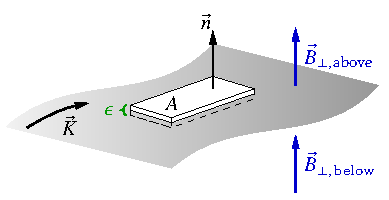
\includegraphics[width=0.45\textwidth,page=1]{pictures/gauss_pillow_magnetic.pdf}}%
    \hspace*{0.1\textwidth}%
    \subfloat{\includegraphics[width=0.45\textwidth,page=2]{pictures/gauss_pillow_magnetic.pdf}}

    \caption{Heavily inspired by Figs.~5.49, 5.50 in \cite{Griffiths_2017}. Note that $\vec{B}_{\perp, \parallel}$ are meant to be the fields in the immediate (in fact, infinitesimal) vicinity of the surface.}
    \label{fig:gaussian_pillow_magnetic}
\end{figure}



for magnetic field, however, Maxwell equations are reversed in which one is zero and which one non-zero, and so are the boundary conditions:
\begin{equation}
    \eqbox{
        B_{\perp, \text{above}} = B_{\perp, \text{below}}
    }
\end{equation}
(since $\oint \vec{B} \cdot d\vec{\mathcal{S}} = 0$)


\begin{equation}
    \eqbox{
        \vec{B}_{\parallel, \text{above}} - \vec{B}_{\parallel, \text{below}} = \mu_0 \vec{K}_f \cross \vec{n}
    }
    \quad \Leftrightarrow \quad
    \eqbox{
        B_{\parallel, \text{above}} - B_{\parallel, \text{below}} = \mu_0 K
    }
\end{equation}
(since $\oint \vec{B} \cdot d\mathcal{C} = B_{\parallel, \text{above}} l - B_{\parallel, \text{below}} l = \mu_0 I_{\mathcal{C}} = \mu_0 K l$)
-> now it is parallel component that is discontinuous (comes from fact that cross products are now involved)


all in one equation:
\begin{equation}
    \eqbox{
        \vec{B}_\text{above} - \vec{B}_\text{below} = \mu_0 \vec{K} \cross \vec{n}
    }
\end{equation}


again, potential is continuous (assuming $\vec{A}$ is divergence-free)
\begin{equation}
    \eqbox{
        A_\text{above} = A_\text{below}
    } \, ,
\end{equation}
but its derivative is not:
\begin{equation}
    \eqbox{
        \pdv{A_\text{above}}{n} - \pdv{A_\text{below}}{n} = - \mu_0 \vec{K}
    } \, ,
\end{equation}



        \subsection{Multipole Expansion}
When dealing with the scalar potential $\varphi$, one of the interesting things that we did was expand the factor $\frac{1}{\norm{\vec{r} - \vec{r}'}}$ in what we called \enquote{multipole expansion}. But the vector potential coming from some volume $\mathcal{V}'$ that contains a current density $\vec{j}(\vec{r}')$,
\begin{equation*}
    \vec{A}(\vec{r}) = \fpmu \int_{\mathcal{V}'} \frac{\vec{j}(\vec{r}')}{\norm{\vec{r} - \vec{r}'}} \, d\mathcal{V}' \, ,
\end{equation*}
contains the same factor, so nothing prevents us from doing the same expansion. We obtain (using Eq.\eqref{eq:multipole_exp_general})
\begin{align}\label{eq:multipole_exp_vectorpot}
    \eqbox{
        \vec{A}(\vec{r})
    }
    % &\simeq \fpmu \int_\mathcal{V} \vec{j}(\vec{a}) \qty[\frac{1}{r} + \frac{\vec{r} \cdot \vec{a}}{r^3} + \frac{3 (\vec{r} \cdot \vec{a})^2 - r^2 a^2}{2 r^5}] d^3a
    &\simeq \fpmu \int_{\mathcal{V}'} \vec{j}(\vec{r}') \qty[\frac{1}{r} + \frac{\vec{r} \cdot \vec{r}'}{r^3}] d\mathcal{V}'
    \\
    &= 
    \eqbox{
        % \fpmu \qty[\frac{\vec{r} \cdot \vec{p}}{r^3} + \frac{1}{2} \sum_{i, j} \frac{Q_{ij}}{r^5} \vec{r}_i \vec{r}_j]
        \fpmu \qty[\frac{\vec{r}}{r^3} \cdot \int_{\mathcal{V}'} \vec{r}' \vec{j}(\vec{r}') \, d\mathcal{V}']
    }
\end{align}
since the monopole term vanishes,
\begin{equation}\label{eq:magn_monopole_term}
    \eqbox{
        \int_{\mathcal{V}'} \vec{j}(\vec{r}') d\mathcal{V}'
        = \frac{1}{r} \underbrace{\int_{\mathcal{V}'} \vec{j}(\vec{r}') d\mathcal{V}'}_{= 0}
        = 0
    }
\end{equation}
(as it should, since there are no magnetic monopoles, but this can be shown in a rigorous calculation).\footnote{Key in the calculation of the dipole term is the identity
\begin{equation}\label{eq:magn_dipole_identity}
    \eqbox{
        \int_{\mathcal{V}'} \vec{a} \cdot \vec{r}' \vec{j}(\vec{r}') \, d\mathcal{V}'
        = - \frac{1}{2} \vec{a} \cross \int_{\mathcal{V}'} \vec{r}' \cross \vec{j}(\vec{r}') \, d\mathcal{V}'
        = \frac{1}{2} \qty[\int_{\mathcal{V}'} \vec{r}' \cross \vec{j}(\vec{r}') \, d\mathcal{V}'] \cross \vec{a}
    } \, ,
\end{equation}
which holds for arbitrary vectors $\vec{a}$.} Note that this integral vanishes no matter the $\mathcal{V}'$ we look at, in particular for a closed tube of infinitesimal diameter (closed is important here, otherwise this is not a connected volume), i.e.~a filamentary current,
\begin{equation}
    \eqbox{
        \oint_{\mathcal{C}'} \vec{j}(\vec{r}') \, d\mathcal{C}' = \oint_{\mathcal{C}'} d\vec{I}' = 0
    } \, ,
\end{equation}
which can be seen as a reflection of the fact no magnetic monopoles exist.

Back to actual expression now. It is only seldomly the case that the dipole term vanishes, so let us focus on this one and omit any higher-order terms. Using some mathematical manipulations, one can rewrite it as
\begin{equation}
    \eqbox{
        \vec{A}_\mathrm{dip}
        = \fpmu \frac{\vec{r}}{r^3} \int_{\mathcal{V}'} \vec{r}' \vec{j}(\vec{r}') \, d\mathcal{V}'
        \underset{\text{Eq.~\eqref{eq:magn_dipole_identity}}}{=} \fpmu \frac{\vec{m} \cross \vec{r}}{r^3}
    }
\end{equation}
with the \Def{magnetic dipole moment}
\begin{equation}\label{eq:magn_dipole_moment}
    \eqbox{
        % \vec{m} = \frac{1}{2} \int_{\mathcal{C}'} \vec{r}' \cross \vec{j}(\vec{r}') \, d\mathcal{C}'
        \vec{m} = \frac{1}{2} \int_{\mathcal{V}'} \vec{r}' \cross \vec{j}(\vec{r}') \, d\mathcal{V}'
    } \, .
\end{equation}
% \todo{here I have discrepancy between previous notes and Griffiths (I have a $\frac{1}{2}$)... translates to result for current loop, $\vec{m} = I \vec{S}$ is Griffiths result; interpretation is supposed to be relation to area in both cases, but I have additional $\frac{1}{2}$ here as well...} -> ah, Griffiths 5.90 is same formula
(Note that, just like the electric dipole moment, this does not depend on position. Once we specify some configuration, $\vec{m}$ is specified. It is easy to get caught up in all the integrals, but nothing in $\vec{m}$ leaves a dependence on position.) If we take as source an Amperian loop (whence integration $\mathcal{V}'$ must be replaced by integration over $\mathcal{C}'$), the dipole moment takes the form $m = I \mathcal{S}$, where $I$ is the current in the loop and $\mathcal{S}$ the area covered by it (i.e.~the area enclosed by $\mathcal{C}$).


-> once again, dipole formula is only exact formula for $\vec{A}$ if loop size goes to zero, while current goes to infinity (so that $m = I a$ remains finite); but in practice, $r \gg a$ is sufficient to invoke dipole form


-> interesting: as Eq.~(5.88) shows, dipole term (and thus far-field limit) of both magnetic potential and field induced by a dipole looks identical to electric dipole (cf.~Eq.~\eqref{eq:el_dipole_field} and Fig.~\ref{fig:magn_dipole})



\begin{figure}
    \centering

    \subfloat[Magnetic Dipole]{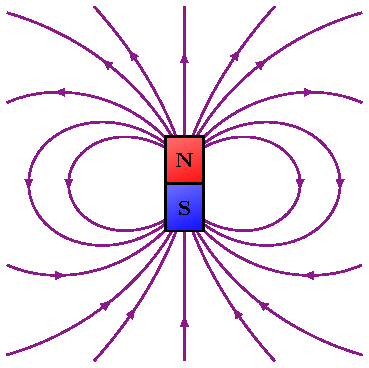
\includegraphics[width=0.4\textwidth]{pictures/magnetic_dipole.pdf}}%
    \hspace*{0.1\textwidth}
    % \subfloat[Electric Dipole]{\includegraphics[width=0.4\textwidth,page=3,angle=0]{pictures/dipole.pdf}}
    \subfloat[Electric Dipole]{\begin{tikzpicture}\node[rotate=-90] at (0,0) {\includegraphics[width=0.4\textwidth,page=3,angle=0]{pictures/dipole.pdf}};\end{tikzpicture}}


    \caption{Comparison of magnetic and electric dipole}
    \label{fig:magn_dipole}
\end{figure}



dipole field:
\begin{equation}
    \eqbox{
        \vec{B}_\mathrm{dip}(\vec{r}) = \fpmu \qty[\frac{3(\vec{m} \cdot \vec{r}) \vec{r}}{r^5} - \frac{\vec{m}}{r^3}]
    }
\end{equation}
(notice how \emph{both} terms scale as $\frac{1}{r^3}$, there is no difference in hierarchy between the two)



Using the same assumption that $\vec{j}(\vec{r}) \neq 0$ only in a small region around some point $\vec{r}_0$ (which is why the Taylor-expansion leading up to Eq.~\eqref{eq:multipole_exp_vectorpot} is warranted), the magnetic field that this region experiences only deviates to first order. This can be used to Taylor-expand the magnetic force (note that we must not expand $\vec{j}$, this still changes significantly since it is a current and not something like a charge density)
\begin{align}
    \eqbox{\vec{F}_\mathrm{dip}}
    &= \int \vec{j}(\vec{r}') \cross \vec{B}(\vec{r}') \, d\mathcal{V}'
    \notag\\
    &= \int \vec{j}(\vec{r}') \cross \qty[\vec{B}(\vec{r}_0) + \eval{\grad_{\vec{r}} \vec{B}}_{\vec{r}_0} (\vec{r} - \vec{r}_0)] \, d\mathcal{V}'
    \notag\\
    &= \underbrace{\qty[\int \vec{j}(\vec{r}') \, d\mathcal{V}']}_{= 0, \text{ cf.~Eq.~\eqref{eq:magn_monopole_term}}} \cross \vec{B}(\vec{r}_0) + \int \vec{j}(\vec{r}') \cross \eval{\grad_{\vec{r}} \vec{B}}_{\vec{r}_0} (\vec{r} - \vec{r}_0) \, d\mathcal{V}'
    \notag\\
    % &= \qty[\qty(\int \vec{j}(\vec{r}') \cross (\vec{r} - \vec{r}_0) \, d\mathcal{V}') \cross \grad] \vec{B}(\vec{r}_0)
    &= \qty[\qty(\int \vec{j}(\vec{r}') \cross \vec{r} \, d\mathcal{V}') \cross \grad - \qty(\qty(\int \vec{j}(\vec{r}') \, d\mathcal{V}') \cross \vec{r}_0) \cross \grad] \vec{B}(\vec{r}_0)
    \notag\\
    \underset{\text{Eqs.~\eqref{eq:magn_dipole_moment}, \eqref{eq:magn_monopole_term}}}&{=} \qty[\vec{m} \cross \grad] \vec{B}(\vec{r}_0)
    \notag\\
    &= - \vec{m} \cdot \qty(\div \vec{B}(\vec{r}_0)) + \grad \qty(\vec{m} \cdot \vec{B}(\vec{r}_0))
    \notag\\
    &\eqbox{= \grad \qty(\vec{m} \cdot \vec{B}(\vec{r}_0))}
\end{align}


-> again, completely analogous to electric dipole; is conservative force with potential
\begin{equation}
    \eqbox{
        V_\mathrm{dip} = - \vec{m} \cdot \vec{B}
    }
\end{equation}
(which resembles potential energy that magnetic field adds to dipole); moreover, since magnetic moment of a specified body does not depend on position, for uniform magnetic fields there is no force on a dipole

-> this yields torque (about the center of the dipole)
\begin{equation}
    \eqbox{
        \vec{M}_\mathrm{dip} = \vec{r} \cross \vec{F}_\mathrm{dip} = \vec{m} \cross \vec{B}
    }
\end{equation}
which, as we see from $V_\mathrm{dip}$, acts until $\vec{m} \parallel \vec{B}$, i.e.~until the dipole is aligned with the magnetic field



To end this bit on dipoles, here is something curious; the cross product in Eq.~\eqref{eq:magn_dipole_moment} looks remarkably like a very familiar quantity, when we calculate it for a single moving test charge with charge $Q$ and mass $M$ (screw it that this is not strictly part of magnetostatics, this is just meant to be a nice demonstration):
\begin{equation}\label{eq:dipole_ang_mom}
    \eqbox{\vec{m}} = \frac{1}{2} \vec{r}_0 \cross Q \vec{v}_0 = \frac{Q}{2 M} \, \vec{r}_0 \cross M \vec{v}_0 = \eqbox{g \vec{L}}
\end{equation}
with the \Def{gyromagnetic ratio}
\begin{equation}\label{eq:gyromagnetic_ratio}
    \eqbox{
        g = \frac{Q}{2 M}
    } \, ,
\end{equation}
an important quantity for particles. It determines how large the dipole moment generated by a charged particle with given angular momentum is. (It should not be surprising \emph{that} a charged particle with angular momentum produces some kind of magnetic field, after all it describes a current. However, the fact that we can relate it directly to a dipole moment, and the fact that the strength relates charge to mass, out of all quantities, are both quite remarkable features, in my opinion.)




        \subsection{Magnetostatics in Matter}
For electrostatics, it was clear how materials can potentially interact with the corresponding fields, since atoms consist of charged particles. If we think about it, the same is true for magnetostatics: we can picture an atom as electrons orbiting the core, which means there are inherently currents when atoms are present.\footnote{Well, quantum mechanics disagrees with this picture; but it still predicts atoms to have magnetic moments, so painting this picture is good enough for this introduction.} For most materials you find in the wild, the only reason that we do not see the magnetic fields produced by atoms is that they are randomly oriented throughout the material, so their net field averages out and is zero. Only if we apply an external magnetic field, we observe a net effect.



            \paragraph{Single Atoms}
Such a net effect can be explained, again, by modelling each atom as a small magnetic dipole. We have derived the force and torque on a magnetic dipole, so we are equipped to study the different phenomena for different kinds of atoms. A general term for any effect of external magnetic fields on materials is \Def{magnetization} (which is nothing but magnetic polarization).


-> magnetism mainly comes in three different forms and shapes:
\begin{itemize}
    \item Paramagnetism: mechanism responsible for effect is indeed dipoles aligning with external magnetic field; in particular, the resulting dipole moment points in the direction of the external field
    
    -> however, this is not from electron orbiting the core, but rather from the electron's spin; the electron is not actually spinning (how should a point spin?), but from quantum mechanics we know that this quantity named spin does behave like an angular momentum (and in particular, there is a gyromagnetic ratio associated with it); thus, by Eq.~\eqref{eq:dipole_ang_mom} they also have a dipole moment
    

    \item Diamagnetism: effect more complicated, no alignment here; basically, if we model electron as spinning around core, then presence of magnetic field (and associated torque) increases speed of rotation -- a little bit
    
    -> typically much weaker than paramagnetism, so only occurs when paramagnetic effects are not present (typically means we need atoms with even number of atoms)

    -> however, it is an effect that is present in \emph{all} atoms, unlike paramagnetism

    -> interesting: it causes magnetic dipole moments that point \emph{opposite} of the magnetic field
    

    \item Ferromagnetism: most prominently iron (in fact, name is derived from latin word for iron)
    
    -> based on effect mentioned in paramagnetism (i.e.~electron spins), but very different from other magnets in that neighbor interactions play a role (it is thus frequently studied in statistical mechanics, e.g., as part of the Ising model)
    
    -> dipoles all align in certain areas, but material has many of such areas, which in turn have random orientation; therefore, initially, there is no net field; but as soon as we put on external field, the different domains begin to align with this external field; this process begins at the domain walls, the dipoles there are competing against each other, but chances are better for boundaries where dipoles are aligned with external field; others will follow boundary, i.e.~the domains merge together, and if we do this long enough the result is essentially one large domain with a really strong magnetic field (the state of \Def{saturation} is reached)

    -> material undergoes some kind of phase transition; this process is actually irreversible (or at least: hardly; we have to play with things like temperature to get something done here), at least getting back the initial state with random orientations; we can only move between different states on what is called \Def{hysteresis curve/loop} -- but I want go into much further detail here, this is already too much statistical mechanics here
\end{itemize}

-> ferro is \emph{much} stronger, we are talking about orders of $10^4 - 10^5$



            \paragraph{Overall Effect}
Materials where atoms align (in whatever manner) in an external magnetic field become \Def{magnetized}, i.e.~they form their own magnetic field. Proceeding in complete analogy to electric fields in matter (the story from the magnetic dipole discussion continues), one defines the \Def{magnetization}\footnote{Here we stick to $\vec{M}$, which has already been used for torques. At least we can make sense of the naming here, after all it is the starting letter of the effect it describes...}
\begin{equation}
    \vec{M} \coloneqq \text{(average) magnetic dipole moment per volume} \, .
\end{equation}

-> for para- and diamagnetic materials, effect of magnetization is often so small that it an safely be neglected; but here is what effect is, in principle: paramagnets are attracted by/into the field, diamagnets are repelled


The total vector potential generated by $\vec{M}$ is easily calculated because magnetic fields obey the superposition principle, so we can just integrate over all the tiny dipole fields:
\begin{equation}
    \vec{A}(\vec{r}) = \fpmu \int_{\mathcal{V}'} \vec{M}(\vec{r}') \cross \frac{\vec{r} - \vec{r}'}{\norm{\vec{r} - \vec{r}'}^3} \, d\mathcal{V}' \, .
\end{equation}
However, we can again invest some of our time to rewrite this and obtain a physically more meaningful expression (the usual steps are involved; product rule, some variant of the generalized Stokes theorem...):
\begin{equation}
    \eqbox{
        \vec{A}(\vec{r}) = \fpmu \int_{\mathcal{V}'} \frac{1}{\norm{\vec{r} - \vec{r}'}} \underbrace{\grad' \cross \vec{M}(\vec{r}')}_{\eqqcolon \vec{j}_b} \, d\mathcal{V}'
        + \fpmu \oint_{\mathcal{S} = \partial \mathcal{V}} \frac{1}{\norm{\vec{r} - \vec{r}'}} \underbrace{\vec{M}(\vec{r}') \cross \vec{n}_{\mathcal{S}}}_{\eqqcolon \vec{K}_b} \, d\mathcal{S}
    } \, .
\end{equation}
The potential of a magnetized object is due to a volume current $\vec{j}_b$ in the material and a surface current $\vec{K}_b$ on its surface. It is now \Def{bound currents} that produce an effect, akin to bound charges in the electric field case.

-> how do these bound currents come to be? Are they just mathematical trick? Again, no. Fig.~6.15 in Griffiths is brilliant on that: for many small dipole currents in the material, most of them will cancel because (for pair of atoms) left has current up in same place where right has current down, so there is no net effect; but what about at the boundary? There we have no cancellation, which leads to a surface current from each atom; total surface current of them precisely comes out to be $\vec{K}_b = \vec{M} \cross \vec{n}$; volume currents can be induced if the internal currents do not cancel completely -- which is very much possible, namely when the magnetization is non-uniform (meaning the dipole currents vary, even from atom to atom, if just ever so slightly), and again we can heuristically show that such a current has the form $\vec{j}_b = \curl \vec{M}$ (fun fact: $\div \vec{j}_b = 0$, as expected for a steady current)



            \paragraph{Modified Maxwell Equations}
So, wow does the total macroscopic field in presence of magnetized material look like? The total current density gets two contributions, from bound and free ones, i.e.
\begin{equation}
    \vec{j} = \vec{j}_b + \vec{j}_f \, .
\end{equation}
Ampere's law, encompassing the source of magnetic fields, then reads
\begin{equation}
    \frac{1}{\mu_0} \curl \vec{B} = \vec{j} = \vec{j}_b + \vec{j}_f = \curl \vec{M} + \vec{j}_f
\end{equation}
(Inverse of $\mu_0$ should not be surprising, it was multiplied in Biot-Savart, unlike $\epsilon_0$. This inverse role just continues, but also: who cares? It is just a constant.) The quantity sourcing free currents is
\begin{equation}
    \eqbox{
        \vec{H} \coloneqq \frac{1}{\mu_0} \vec{B} - \vec{M}
    }
\end{equation}
an auxiliary field $\vec{H}$\footnote{You might have expected a name here, maybe something along the lines of \enquote{magnetic displacement}. But Griffiths says $\vec{H}$ has no sensible name (cf.~page 282) and I will not argue with him on such things.}, i.e.
\begin{equation}
    \eqbox{
        \oint \vec{H} \cdot d\vec{\mathcal{C}} = I_{f, \mathcal{C}}
    } \, .
\end{equation}

-> very interesting take: while $\vec{D}$ is more of a helper quantity, $\vec{H}$ is actually more useful in a lab than $\vec{B}$ in many cases; reason is of practical nature: we often generate magnetic fields using electromagnets, meaning it is $\vec{H}$ that we source; meanwhile, we create electric fields via voltages = potential differences, so here it is $\vec{E}$ that we source; still, from a purely theoretical perspective, the quantities on equal footings from their role in electromagnetism are $\vec{E} \leftrightarrow \vec{B}, \vec{D} \leftrightarrow \vec{H}$


-> careful, no free current does not imply $\vec{H} = 0$; while curl vanishes, divergence does not (so via Helmholtz the field does not; at least not trivially, integral can of course still conspire to give zero) since $\div \vec{H} = - \div \vec{M}$



            \paragraph{Linear Media}
For many (most) materials, magnetization is always proportional to the total magnetic field (This cannot exclude ferromagnets since they retain a magnetization even if we remove the external field again; but ferromagnets are also not \enquote{most materials}.) We are thus tempted to write
\begin{equation}
    \vec{M} = \frac{1}{\mu_0} \chi_m \vec{B}
\end{equation}
for an appropriate constant $\chi_m$. However, this is one of the few places where the electric and magnetic treatment differ; \Def{magnetic susceptibility} $\chi_m$ is defined as a dimensionless quantity via
\begin{equation}
    \eqbox{
        \vec{M} = \chi_m \vec{H}
    }
\end{equation}
and thus in terms of the field generated by the free currents. (Typical magnetic susceptibilities are on the order of $10^{-4}$. They are $< 0$ for diamagnets and $> 0$ for paramagnets.) The total magnetic field for linear media reads
\begin{equation}
    \eqbox{\vec{B}} = \mu_0 (\vec{H} + \vec{M}) \eqbox{= \mu_0 (1 + \chi_m) \vec{H} \eqqcolon \mu \vec{H}}
\end{equation}
with the material's \Def{permeability} $\mu$ and \Def{relative permeability} $\mu_r$.



            \paragraph{Boundary Conditions}
Again we are interested in rewriting the boundary conditions in terms of the free currents and the related quantity $\vec{H}$. The same procedure as before leads to
\begin{equation}
    \eqbox{
        H_{\perp, \text{above}} - H_{\perp, \text{below}} = - (M_{\perp, \text{above}} - M_{\perp, \text{below}})
    }
\end{equation}
and
\begin{equation}
    \eqbox{
        \vec{H}_{\parallel, \text{above}} - \vec{H}_{\parallel, \text{below}} = \vec{K}_f \cross \vec{n}
    }
\end{equation}


In homogenous linear media, we can simplify a little bit since
\begin{equation}
    \eqbox{
        \vec{j}_b = \curl \vec{M} = \curl (\chi_m \vec{H}) = \chi_m \vec{j}_f
    } \, .
\end{equation}
One interesting consequence of this expression is that, if the free current does not penetrate into the material, bound current can only be at the surface (which is only place that free current can reach, if it is not in the body). The divergence of $\vec{M}$, however, does still not vanish in general (due to problems at the boundary).



    \section{Electrodynamics}
Now that we impose no restrictions on the configuration of charges, we have to study a few more interactions in addition to those that have been treated already. Our expectation is that electric and magnetic field are gonna mix, as we have already seen in example \ref{ex:point_charge_magn_field} with point charges, simply because we can now have non-vanishing charge and motion of said charge at the same time.



In statics, the electric field is curl-free and the magnetic field is divergence-free. As we will see, this changes when looking at electrodynamics, and not just that, there will be a mixing and interaction of electric, magnetic field. More detailed analyses of the interplay between the two fields, and especially a relativistic treatment, then reveals that the two are manifestations of one and the same phenomenon, an electromagnetic field. The electric (magnetic) field only arise in the special cases of electro(magneto-)statics as the curl-(divergence-)free components of this electromagnetic field.


We can already see that the lines between electric and magnetic fields are actually more blurry than they seem by studying a very simple example, the interaction of two moving point charges. (Note that this is neither a problem from electrostatics nor from magnetostatics, since there are both net charges and currents in this setup. Thus it falls into the realm of electrodynamics).

% -> basically: is due to length contraction, moving charge sees different distribution of charges than resting. Historical approach: introduce new field and force, magnetic field. This complements electrical interaction between two charges, both of which are moving.

% -> better wording: can be analyzed/explained entirely by a proper relativist analysis of the situation. Results match what was found empirically be Biot and Savart


% From a modern perspective, with relativity theory developed (this was not the case when these effects were found), it would be straightforward to look at electric field in rest frame of charges moving in the current and then transform back into an \enquote{external}, inertial frame. Historically speaking, however, relativity theory was not there when the aforementioned effect was discovered. Therefore, it was the most natural thing to associate it with new physics, and this is how the \Def{magnetic field} came into existence.
% \footnote{For a very clear, yet concise derivation of the laws of electromagnetism from Coulomb's law (i.e.~electrostatics), see this article by Leigh Page: \url{https://zenodo.org/record/1450178}.}



\begin{ex}[Two Moving Point Charges]\label{ex:point_charge_magn_field}
    Verbally/In words, I can claim a lot, for instance that electric and magnetic field are essentially the same thing viewed from different frames, but do these claims hold up when looking at actual expressions? For that, let us look at the simples scenario possible, the force between two currents made up of a single test charge each, i.e.~$\vec{j}_i = q_i \vec{v}_i \, \delta (\vec{r} - \vec{r}_i)$. In that case, the Biot-Savart law reads
    \begin{equation}
        \vec{B}_1(\vec{r}) = \fpmu q_1 \vec{v}_1 \cross \frac{\vec{r} - \vec{r}_1}{\norm{\vec{r} - \vec{r}_1}^3}
    \end{equation}
    and the corresponding Lorentz force exerted on the second particle becomes
    \begin{align}
        \vec{F} &= q_2 \vec{v}_2 \cross \vec{B}(\vec{r}_2) = \fpmu \frac{q_1 q_2}{\norm{\vec{r}_2 - \vec{r}_1}^3} \vec{v}_2 \cross \qty[\vec{v}_1 \cross (\vec{r}_2 - \vec{r}_1)]
        \notag\\
        &= \fpmu \frac{q_1 q_2}{\norm{\vec{r}_2 - \vec{r}_1}^3} \qty[(\vec{v}_2 \cdot (\vec{r}_2 - \vec{x_1})) \vec{v}_1 - (\vec{v}_2 \cdot \vec{v}_1) (\vec{r}_2 - \vec{r}_1)]
        \notag
    \end{align}
    If you are trained in relativity, then you will recognize that does look a lot like a Lorentz transform (even more so since $\mu_0 = \frac{1}{c^2 \epsilon_0}$). To see this in even more detail, let us assume that $\vec{v}_1 \parallel \vec{v}_2 \parallel \vec{e}_x$ while the displacement vector is $\vec{r}_2 - \vec{r}_1 \parallel \vec{e}_y$. In that case,
    \begin{align}
        \vec{F} &= \fpmu \frac{q_1 q_2}{\norm{\vec{r}_2 - \vec{r}_1}^3} \qty[(\vec{v}_2 \cdot (\vec{r}_2 - \vec{x_1})) \vec{v}_1 - (\vec{v}_2 \cdot \vec{v}_1) (\vec{r}_2 - \vec{r}_1)]
        \notag\\
        &= - \frac{v_1 v_2}{c^2} \fpeps q_1 q_2 \frac{\vec{r}_2 - \vec{r}_1}{\norm{\vec{r}_2 - \vec{r}_1}^3}
        \notag
    \end{align}
    However, this is not the total Lorentz force yet. Since there is only one test particle for each current in this setup, the electric field is not vanishing. Therefore, the Coulomb force between the particles is also acting and due to the superposition principle for forces, we can simply add the term $q \vec{E}_1(\vec{r}_2)$ to $\vec{F}$, which yields the total Lorentz force
    \begin{equation}
        \vec{F} = \fpeps q_1 q_2 \frac{\vec{r}_2 - \vec{r}_1}{\norm{\vec{r}_2 - \vec{r}_1}^3} - \frac{v_1 v_2}{c^2} \fpeps q_1 q_2 \frac{\vec{r}_2 - \vec{r}_1}{\norm{\vec{r}_2 - \vec{r}_1}^3} = \fpeps q_1 q_2 \frac{\vec{r}_2 - \vec{r}_1}{\norm{\vec{r}_2 - \vec{r}_1}^3} \qty(1 - \frac{v_1 v_2}{c^2})
        \notag\, .
    \end{equation}
    where we have further simplified the setup by choosing the test charges to be exactly co-moving, $v_1 = v_2$.\footnote{Granted, this step is mostly done to arrive quickly at a convenient expression, but in my understanding, this simply avoids doing two Lorentz transforms because for $v_1 = v_2$, the rest frame of both test charges is the same. A justification of this is given by the existence of general treatments, which we mention later on.} This equation can be further rewritten by making use of the Lorentz factor $\gamma = (1 - v^2 / c^2)^{-1/2}$:
    \begin{equation}
        \eqbox{
            \vec{F} = \fpeps q_1 q_2 \frac{\gamma(\vec{r}_2 - \vec{r}_1)}{\gamma^3 \norm{\vec{r}_2 - \vec{r}_1}^3}
        }
        \, .
    \end{equation}
    -> some more stuff goes into this (perhaps already in equation before); we assume that difference only has non-zero components in direction that particles move (otherwise gamma in front of vector difference does not work); is fine, but must be mentioned -> actually this might not even be the case

    -> mention that even in non-relativistic case we get correct result -> ah, but then we have electric field mostly... This is difference to Feynman lecture example, where no net charge, so that B-field is \emph{only} field left (then the argument of \enquote{electric interaction so strong that this tiny length contraction has effect even for non-relativistic speeds} makes sense, here not so much)

    Therefore, we see that the Lorentz force exerted in a frame relative to which the point charges move is essentially a boosted version of the Lorentz force in a frame where the charges are stationary. Length contraction changes how the field is perceived in this frame. Granted, we have made many simplifying assumptions here (and also look only at the three-vector $\vec{F}$ here), but sources like \cite{Rosser_1968}, Chapter 3., or \cite{Page_1912} show how this can work in very general setups. Our treatment is merely meant to be an outline of the general strategy used to show the acclaimed equivalence.

    \todo{is this really what we intend to show?} -> yes, it is; from inertial frame with respect to which the charges are moving, it looks like the two charges are interacting via Coulomb force over distance $\norm{\vec{r}_2 - \vec{r}_1}$, and the associated currents are interacting via magnetic force over the same distance; however, what we see upon rewriting is that the total Lorentz force is just a Coulomb force, but acting over a contracted distance $\norm{\vec{r}_2 - \vec{r}_1}$ (analyzing from the rest frame, this is the value that the moving charges measure for their separation)

    \todo{draw simply TikZ plot of situation?}



    \todo{mention Griffiths Eq.~(5.43), which is non-relativistic limit; this is version obtained from Biot-Savart, so Biot-Savart is approximately correct even for electrodynamics, if relativistic effects are not pronounced}
\end{ex}
To summarize this example, relativity shows in quite natural (and, arguably, quite elegant) manner that electric and magnetic force are manifestations of the same phenomenon. It unifies the treatment of problems involving charges and explains different contributions, e.g., to the Lorentz force. So, why does the majority of textbooks still take the approach to explain them separately? Well, in the end still kind of independent because we can treat as separate effects (though mixing is frame-dependent)

-> still makes sense to treat separately, what we have here is really mainly due to movement (as initial thought experiment shows), so the two manifestations occur in independent setups (though, of course, one can have both at a time; this is realm of electrodynamics)



        % \subsection{Electromotive Force \& Induction}
        \subsection{Electromotive Force}
On our way towards electrodynamics, it is crucial to understand the interplay between charges and currents. A natural first question in this context is: how can we even create a current, i.e.~how can we get charges into motion? Well, the answer is not too hard: by exerting a force on them. Therefore, we can write down the general expression
\begin{equation}\label{eq:ohm_law_generalized}
    \eqbox{
        \vec{j} = \sigma \vec{f}% = \frac{1}{\rho} \vec{f}
    }
    \quad \Leftrightarrow \quad
    \eqbox{
        \vec{f} = \rho \vec{j}
    }
\end{equation}
with a force per unit charge $\vec{f}$. We have shown two ways in which this proportionality may be expressed; the one involving the \Def{conductivity} $\sigma$ is more straightforward to write down, but numbers are usually given for its inverse, the \Def{resistivity} $\rho = \frac{1}{\sigma}$ (these two have \emph{nothing} to do with charge or surface density; these are just more symbols that are used multiple times).


In case we use the electromagnetic (Lorentz) force to move the charges, this equation becomes
\begin{equation}\label{eq:ohm_law}
    \eqbox{
        \vec{j} = \sigma (\vec{E} + \vec{v} \cross \vec{B}) \approx \sigma \vec{E}
    }
\end{equation}
which is known as \Def{Ohm's law}. (We have used that the magnetic contribution is much smaller for the far from relativistic velocities that charges usually move with; this is not valid if we aim to analyze plasmas for instance.)

In conductors, where the number of available charges is practically infinite, $\sigma = \infty$ implies $E = J / \sigma = 0$ no matter if a current is present or not (i.e.~even in electrodynamics, there is no electric field in conductors). It is for this reason that wires in electric circuits are often treated as lossless, i.e.~as equipotentials. Resistors, on the other hand, do not conduct well ($\rho$ large $\Leftrightarrow \sigma$ low), so that large fields are required to produce a significant current.


A note on Ohm's law: it is not a \enquote{law} in the truest sense, meaning it does not hold on the same level as, e.g., Coulomb's law. It just happens to be a relationship that holds reasonably well for practical calculations (we can see it as macroscopic formula that neglects microscopic physics, or rather assumes it can be encapsulated in macroscopic constants like the conductivity).



\begin{ex}[Ohm's Law]
    You may be familiar with a different form of Ohm's law, $U = R I$. And while Eq.~\eqref{eq:ohm_law} may not look exactly like that, we can see the equivalence in a special case, namely when we look at the current flowing through a body of length $L$ with area $A$ perpendicular to $L$

    -> important property (not trivial, this one must prove; uniqueness theorem is helpful here, as virtually always -> details in Griffiths Ex.~7.3, where field is even calculated explicitly): field through the body is constant, and by Ohm's law so is the current

    -> total current through surface with area is simply $I = j A$ ($j$ constant)

    -> we know that $\int_0^L \vec{E} \cdot d\vec{r} = \varphi_L - \varphi_0$; the field throughout the volume is constant, so that $\int_0^L \vec{E} \cdot d\vec{r} = E L$; in total, this means
    \begin{equation}
        I = A \sigma \frac{U}{L}
    \end{equation}
    which reads $U = R I$ if we agree to call $\frac{L}{A \sigma} \eqqcolon R$ the resistance and denote the voltage between both ends as $U \coloneqq \varphi_L - \varphi_0$

    resistance is measured in \Def{Ohms} with
    \begin{equation}
        \eqbox{
            1 \unit{\ohm} = 1 \unit{\volt \per \ampere}
        }
    \end{equation}
    -> is a geometrical quantity that encapsulates the geometry of the shape and its material properties (conductivity)

    -> this is interesting because it means that I can double current flow between capacitor plates with conducting material between them (as example) by doubling charge on the plates (which doubles electric field and thus also potential)


    -> main effect of non-zero resistance: work done by electric field is lost (converted to heat in the resistor, through collisions of charges with particles of medium);
    % we have the work done by an electric field on a charge $q$ in Eq.~\eqref{eq:work_test_part_1}, it is $W = q U$; but here we do not have a single $q$, but rather a charge density
    the work done per unit volume $d\mathcal{V}$ (must be used here, there is not a single charge; we look at force on $\rho d\mathcal{V}$) is
    \begin{equation}
        dW_{\mathcal{V}} = \rho d\mathcal{V} \, \vec{E} \cdot d\vec{r} = \rho d\mathcal{V} \, \vec{E} \cdot \vec{v} dt = \vec{E} \cdot \vec{j} d\mathcal{V} dt
    \end{equation}
    this equation is still generally applicable; for special case of constant current and electrical field (which are also parallel, by Eq.~\eqref{eq:ohm_law_generalized}), the power (or rather: power loss) is
    \begin{equation}
        \eqbox{P}
            = \dv{W}{t} = E j V = E j (L A) \eqbox{= U I = R I^2 = \frac{U^2}{R}}
    \end{equation}
    this equation is called \Def{Joule heating law}

    -> unit of power is the old familiar \Def{Watts} with
    \begin{equation}
        1 \unit{\watt} = 1 \unit{\joule \per \second} \, ,
    \end{equation}
    just as in Newtonian physics
\end{ex}


-> another interesting consideration: say the conductivity is uniform (otherwise arbitrary) and all currents are steady. Then, by Ohm's law
\begin{equation}
    \eqbox{
        \div \vec{E} = \div \frac{\vec{j}}{\sigma} = \frac{1}{\sigma} \div \vec{j} = 0
    }
\end{equation}
which implies that there can be no charge density inside the material. Just as was the case in electrostatics, all charges reside on the surface. Therefore, it is Laplace's equation that may be solved in a homogenous material with ohmic resistance, not Poisson's and all the machinery for that may be used.



We have asked ourselves how to produce a current and found that it can be produced by pushing charges around, i.e.~applying a force to them. In an electric circuit, this \enquote{pushing} is done by devices like batteries. But batteries are only connected to the two ends of the circuit, so the only place where a force is applied by them is on those two ends and inside the battery itself. That means we are able to calculate the current only in those places, but not the rest of the circuit. Right?

Actually, we are lucky and there is an automatic feedback built into circuits. Suppose we have some current $\vec{j}_s \coloneqq \vec{j}_\text{source}$ in the battery and some other current $\vec{j}_o \coloneqq \vec{j}_\text{other}$ elsewhere in the circuit. With $j_s$ being larger than $j_o$, it is clear that the charge density must vary throughout the circuit (charges flow faster inside the battery). However, this produces an electric field. Say the current in the battery flows from left to right, so that there are more positive forces on the right side of the battery; then this accumulation of positive charges induces an electric field that points to the \emph{left}, i.e.~opposite of the current flow. This results in the current flow slowing down, allowing the charge accumulation to slowly flow away; this results in a decrease of the opposed electric field, and the net result is an equilibrium where $j_s = j_o$. In other words, the current throughout the whole circuit is the same. This automatic feedback happens extremely fast in reality, so that we can always assume that currents are the same throughout a circuit.


This process is very interesting (and in fact, beautiful, as it makes the theoretical analysis a lot easier), so let us look at it in more detail. Throughout the source, there are two forces that act: $\vec{f}_s$, the force in the source driving the current; and $\vec{E}$, the force one can attribute to any potential difference building up over the circuit (the opposing electric field would contribute to that, in the parts of the circuit where it builds up, but this $\vec{E}$ is more general; note that $\vec{E}$ can be regarded as a force in the sense that $\vec{E} = \vec{F} / q$, which is what we defined $\vec{f}$ as). \cite{Griffiths_2017} uses the nice analogy that $\vec{E}$ is the force that \enquote{smooths out the flow} (i.e.~that ensures $j_s = j_o$, using the terms from above) and thus \enquote{communicates the influence of the source to distant parts of the circuit}. In other words, the total force per unit charge is
\begin{equation}
    \eqbox{
        \vec{f} = \vec{}_s + \vec{E}
    } \, ,
\end{equation}
from which the total force throughout the circuit can be obtained as a line integral
\begin{equation}
    \eqbox{
        \mathcal{E} = \oint \vec{f} \cdot d\vec{r} = \oint \vec{f} \cdot d\vec{r}
    }
\end{equation}
Here we have used the property $\oint \vec{E} \cdot d\vec{r} = 0$ from electrostatics. (It is justified to use electrostatics here because we have already established that the charge density must be constant. Any change in it would immediately be compensated by an increase in the opposing electric field.) Although this is not truly a force (we have integrated a force density per unit charge over a spatial dimension), this quantity is commonly called \Def{electromotive force} (EMF).

The fact that the EMF is not quite a force can also seen by the following consideration. Say our source is ideal, i.e.~there is no net force on charges in it, which is equivalent to $\vec{f}_s = - \vec{E}$. Then the potential difference between the two points $a, b$ at which the source is attached reads
\begin{equation}
    U = - (\varphi_b - \varphi_a) = - \int_a^b \vec{E} \cdot d\vec{r} = \int_a^b \vec{f}_s \cdot d\vec{r} = \oint \vec{f}_s \cdot d\vec{r} = \mathcal{E}
\end{equation}
where we can replace integrating over the source (i.e.~between $a, b$) by integrating over the whole circuit because $\vec{f}_s$ is zero anyway outside of the source. Therefore, the EMF is equal to the voltage between the source ends (which is equal to the voltage going from $b$ to $a$ through the rest of the circuit). In other words, the job of the source is to drive the voltage in the circuit (this is what, e.g., the chemical work done in Lithium batteries is used for). The resulting electric field $\vec{E} = - \vec{f}_s$ then sources the current throughout the rest of the circuit.



            \paragraph{Motional EMFs}
I do not like, skipping most of it for now

-> explains generators, i.e.~what happens when I move wire inside a magnetic field

most important result: \Def{flux rule},
\begin{equation}
    \eqbox{
        \mathcal{E} = - \dv{\Phi}{t}
    }
\end{equation}
where $\Phi$ is the flux of the magnetic field through the loop,
\begin{equation}
    \eqbox{
        \Phi \coloneqq \int_{\mathcal{S}} \vec{B} \cdot d\vec{\mathcal{S}}
    }
\end{equation}

-> can be applied for every possible scenario, even non-uniform magnetic fields and weird wire geometries (need not be rectangular or in specific direction)


-> flux rule is just based on Lorentz force, so in that sense it does not reveal anything new, but it is still a convenient tool for calculations

-> careful, though: flux rule only works for a single wire loop; this loop can be super complicated, weirdly deformed or whatever, but it must be a single one



\begin{ex}[Eddy Currents]
    ugly... But important. they can help us to make effect of magnetic field zero, in case we do not want to have it (by making sure currents generated by different parts of geometry cancel)
\end{ex}



        \subsection{Induction}
Faraday analyzed experimentally the effects of a time-dependent magnetic field and was able to derive the following relationship:
\begin{equation}\label{eq:maxwell_edyn_one_int}
    \eqbox{
        \oint_\mathcal{C} \vec{E} \cdot d\vec{r} = - \int_{\mathcal{S}(\mathcal{C})} \pdv{\vec{B}}{t} \cdot d\vec{\mathcal{S}}
    }
\end{equation}
where $\mathcal{S}(\mathcal{C})$ is the area that is enclosed by $\mathcal{C}$ (equivalently, we could replace $\mathcal{C} \mapsto \partial \mathcal{S}, \mathcal{S}(\mathcal{C}) \mapsto \mathcal{S}$). To honor its discoverer, this equation is also called \Def{Faraday's law}. In differential form, it reads
\begin{equation}\label{eq:maxwell_edyn_one_diff}
    \eqbox{
        \curl \vec{E} = - \pdv{t} \vec{B}
    } \, .
\end{equation}


What the current treatment of the topic does not reveal is that Faraday carried out not one, but multiple experiments playing around with wire loops and magnetic fields. All of them can be explained by a \Def{generalized/universal flux rule} (though the setups are really different for all of them): whenever the magnetic flux throughout a loop changes, an EMF
\begin{equation}
    \mathcal{E} = - \dv{\Phi}{t}
\end{equation}
will appear in the loop; however, in order to use the flux rule, one fundamentally new insight is required: a changing magnetic field induces an electric field (\cite{Griffiths_2017} has some words to say on the term \enquote{induces}, since an electric field being produced by the magnetic one does not tell the whole story). This is the content of what we have termed Faraday's law, since other experiments may be seen as manifestations of the motional EMF. The main reason to mention the other experiments is that the variety of situations involved in them makes it confusing to get signs right. While in principle, we can always deduce them from the definitions made, there is an intuitive rule for this, called \Def{Lenz's law}: quoting \cite{Griffiths_2017}, it states
\begin{center}
    Nature abhors a change in flux.
\end{center}
In terms of current this means that any induced current will flow in such a manner that the change in flux that produced the induced current is opposed (note that Lenz's law is concerned with the direction of the flow, not so much with the magnitude).



            \paragraph{About the Induced Electric Field}
Here is something interesting: if the electric field is produced exclusively by a time-varying magnetic field, with $\rho = 0$, then the equations that determine $\vec{E}$ are Faraday's law and the first Maxwell equation of electrostatics,
\begin{equation}
    \div \vec{E} = 0
    \qquad
    \curl \vec{E} = - \pdv{\vec{B}}{t} \, .
\end{equation}
This is equivalent to the set of equations that dictated magnetostatics, so we can apply all knowledge and intuition we have gained there. For example, we can write down a Biot-Savart like law that determines the electric field as
\begin{equation}
    \vec{E}(\vec{r}) = - \frac{1}{4\pi} \pdv{\vec{B}}{t} \cross \frac{\vec{r} - \vec{r}'}{\norm{\vec{r} - \vec{r}'}^3} \, d\mathcal{V}' = - \frac{1}{4\pi} \pdv{t} \vec{B} \cross \frac{\vec{r} - \vec{r}'}{\norm{\vec{r} - \vec{r}'}^3} \, d\mathcal{V}'
\end{equation}
(with no restriction on the time-dependence of $\pdv{\vec{B}}{t}$). Moreover, the second equality can be restated as an integral equation,
\begin{equation}
    \oint \vec{E} \cdot d\vec{r} = - \dv{\Phi}{t}
\end{equation}
akin to Ampere's law. This gives us a recipe to quickly obtain induced electric fields, if the setup is sufficiently symmetric.


note from Griffiths, page 319: \enquote{I must warn you, now, of a small fraud that tarnishes many applications of Faraday's law: Electromagnetic induction, of course, occurs only when the magnetic fields are changing, and yet we would like to use the apparatus of magnetostatics (Ampère's law, the Biot-Savart law, and the rest) to calculate those magnetic fields. Technically, any result derived in this way is only approximately correct. But in practice the error is usually negligible, unless the field fluctuates extremely rapidly, or you are interested in points very far from the source. Even the case of a wire snipped by a pair of scissors (Prob. 7.18) is static enough for Ampère's law to apply. This régime, in which magnetostatic rules can be used to calculate the magnetic field on the right hand side of Faraday's law, is called quasistatic. Generally speaking, it is only when we come to electromagnetic waves and radiation that we must worry seriously about the breakdown of magnetostatics itself.}



            \paragraph{Inductance}
Magnetic forces between objects are mutual, i.e.~if I have one loop exerting force on another loop, then Newton's third law tells us this other loop the same force onto the first loop.



            \paragraph{Magnetic Field Energy}
-> work that must be done to get current flowing (against) can be regarded as stored in the circuit (released when current is turned off, EMF tries to keep it going)


-> magnetic forces indeed do no work, they merely convert different energies the system has; for example, rotational energy into potential



        \subsection{Ampere's Law -- Revisited}
In magnetostatics, currents are steady and fulfil $\div \vec{j} = 0$, they have no sources on which they originate and end (we only have loops \todo{right?}). In electrodynamics, this need not be true, which poses a problem since
\begin{equation}
    \mu_0 \div \vec{j} = \div \qty(\curl \vec{B}) = 0
\end{equation}
because the curl of a divergence is always zero. Consequently, we must add a term to the left hand side to make it zero. What offers help is the continuity equation. In statics, $\pdv{\rho}{t} = 0$, so we knew that $\div \vec{j} = 0$. But now, the continuity equation implies vanishing of another expression, namely
\begin{equation}
    \div \vec{j} + \pdv{\rho}{t} = \div \vec{j} + \pdv{t} \epsilon_0 \div \vec{E} = \div \qty(\vec{j} + \pdv{\vec{E}}{t}) \, .
\end{equation}
(Here we assume vacuum for now.) The intuitive explanation goes as follows: If there are non-steady currents, then there must also be a change in charge density with divergence equal to the current, i.e.~an electric field that changes in time.

A different reasoning lead Maxwell to the same conclusion: we should add what he called the \Def{displacement current} to Ampere's law.\footnote{The \enquote{displacement} part occurs because more generally, we would have to use $\vec{D}$ here rather than $\vec{E}$, since this is what free charge densities source. For a discussion in vacuum, it is merely a matter of taste if we use $\vec{E}$ or $\vec{D}$}. This modified version,
\begin{equation}
    \eqbox{
        \curl \vec{B} = \mu_0 \vec{j} + \mu_0 \epsilon_0 \pdv{\vec{E}}{t}
    }
\end{equation}
is thus called \Def{Ampere-Maxwell law}. This passes all sanity checks we can come up with; in magnetostatics for example, the additional term vanishes and leaves our existing theory unaffected. In fact, for many experiments with magnetic fields, its impact is negligible (so Faraday's, for instance, never saw this term). But it also makes a bold new prediction: say we have no currents in the volume we analyze, $\vec{j} = 0$. While in statics, this would directly imply $\vec{B} = 0$, now we another source term for magnetic fields: the presence changing electric fields. (Note here that it is truly just the presence. This field need not be produced by charges in the volume $\mathcal{V}$ we are analyzing, yet can still serve as the source of a magnetic field originating from $\mathcal{V}$. Before, we had seen that magnetic fields can extend beyond the volumes occupied by the currents that sourced them; but this is very different, since the magnetic field not just extends into $\mathcal{V}$, it is actually produced there solely because of the changing electric field.) Note also that, although the name \enquote{displacement current} suggests that, this new source has nothing to do with currents except being related to them by the continuity equation (and now by being a source of magnetic fields); but they \emph{are not} currents.


While the validity of this law would introduce a nice duality into the relation of magnetic and electric fields (Faraday's law states that changing magnetic fields produce an electric field), symmetry is not a good argument -- at least not if it contradicts experimental evidence. Here, fortunately, it was experiments conducted by Heinrich Hertz on electromagnetic waves that \emph{confirmed} Maxwell's modification.




% -> when induction stuff is removed: Faraday's law tells us what happens when we have magnetic fields that change in time; what is still missing is the effect of electric fields that change in time -> formally, we can associate with current (via continuity equation); but only insofar as to equality with $\curl \vec{B}$, is not an actual current (although Maxwell gave name that contains current)
% -> why? After all, any change in $\rho$, which is required for change in $\vec{D}$, automatically means charges are moving -- i.e.~a current; right? Yes, this is true; but the changing electric field also propagates further out in space and thus to positions where the motion of charges induced by $\pdv{\rho}{t}$ does not take place; we only feel the \emph{effect} of it, a time-varying electric field; this effect is \emph{akin to} a current, by the continuity equation, but it does not mean there \emph{is} a motion of current that \emph{caused} this.

% -> basically: I experience effect of change in charge density and associated current $\vec{j}_c$ elsewhere too, as change in electric field -- even in places where $\vec{j}_c = 0$; for this reason, we should refrain from thinking about displacement current as an actual current; formally, though, we can associate change in e-field with divergence of current, so we have to account for it as source of b-field -- but this is something new and changes the way we think about b-fields: they are caused by currents and time-varying electric fields (two distinct effects; their identification via continuity is just tool to make sense of derivation; this derivation is not super rigorous, it just happens that this reasoning yields same result that we observe empirically when conducting experiments)


% -> the presence of a time-varying electric field acts as a source for magnetic fields; i.e.~if I enclose an area and it contains currents, then it produces magnetic field; but in just the same manner, if I enclose an area and it contains a time-varying electric field (is possible, even if $\rho = 0$ throughout the area!), then it too produces a magnetic field

% -> we are used to magnetic fields extending out of the region where it is sourced, otherwise how would there be a magnetic force? But here, it not justs \emph{exists} outside of an area where no current is present, it is \emph{produced/sourced} there!


The corresponding integral form is%\todo{verify this equation. I have never seen it anywhere}
\begin{equation}\label{eq:maxwell_edyn_two_int}
    \eqbox{
        \oint_\mathcal{C} \vec{H} \cdot d\vec{r}
        = I + \oint_{\mathcal{S}(\mathcal{C})} \pdv{\vec{D}}{t} \cdot d\vec{\mathcal{S}}
        % = I - \epsilon_0 \pdv[2]{t} \vec{B} + \oint_{\mathcal{S}(\mathcal{C})} \pdv{\vec{\mathbb{P}}}{t} \cdot d\vec{\mathcal{S}}
    }
\end{equation}
where $\mathcal{S}(\mathcal{C})$ is the area that is enclosed by $\mathcal{C}$.



        \subsection{Maxwell Equations}
Interestingly, in order to do time-independent electrodynamics, i.e.~electromagnetism, the only thing we have to do is take the Maxwell equations from electro-, magnetostatics and continue with this set of equations. It is only when we go to dynamics with $\pdv{\vec{E}}{t} \neq 0$ and/or $\pdv{\vec{B}}{t} \neq 0$ that we have to do more work. This work has been done over the past two subsections, which is paying off now because we merely have to assemble the appropriate set of equations.
\todo{uhhh, does this make sense? Is there even something like \enquote{time-independent electrodynamics}?}



            \paragraph{In Vacuum}
In vacuum, Maxwell's equations in their most general form are
\begin{subequations}
\begin{align}
    \div \vec{E} &= \frac{\rho}{\epsilon_0}
    \\
    \div \vec{B} &= 0
    \\
    \curl \vec{E} &= - \pdv{\vec{B}}{t}
    \\
    \curl \vec{B} &= \mu_0 \vec{j} + \mu_0 \epsilon_0 \pdv{\vec{E}}{t}
\end{align}
\end{subequations}
Equivalently, in integral form,
\begin{subequations}\label{eq:maxwell_collection}
\begin{align}
    \int_{\mathcal{S}} \vec{E} \cdot d\vec{\mathcal{S}} &= \frac{Q(\mathcal{V})}{\epsilon_0}
    \\
    \int_{\mathcal{S}} \vec{B} \cdot d\vec{\mathcal{S}} &= 0
    \\
    \int_{\mathcal{C}} \vec{E} \cdot d\vec{\mathcal{C}} &= - \pdv{t} \int_{\mathcal{S}(\mathcal{C})} \vec{B} \cdot d\mathcal{S}
    \\
    \int_{\mathcal{C}} \vec{B} \cdot d\vec{\mathcal{C}} &= \mu_0 I_{\mathcal{C}} + \mu_0 \epsilon_0 \pdv{t} \int_{\mathcal{S}(\mathcal{C})} \vec{E} \cdot d\mathcal{S}
\end{align}
\end{subequations}


-> some interpretations:

the only situation where an electric field can have broken symmetry in the form of vortices is when a time-varying magnetic field is present. This symmetry breaking manifests as non-zero line integrals over a closed path.



            \paragraph{In Media}
Nothing really changes in the form of Maxwell's equations when we make the transition in media, except that $\rho$ and $\vec{j}$ now have multiple contributions.

-> charge density: from free and bound charges, $\rho = \rho_f + \rho_b$

-> current density: also from free and bound charges, $\vec{j} = \vec{j}_f + \vec{j}_b$; but it actually also gets new contribution, from \Def{polarization current} $\vec{j}_p = \pdv{\vec{\mathbb{P}}}{t}$ (can, again, be derived from continuity equation for the flow of bound charge $\rho_b$; nope, the flow of bound charges is \emph{not} related to the bound current via the continuity equation, their origin is very different)


However, it is possible to rewrite them in terms of $\vec{D}, \vec{H}$, which may be a little more convenient if we intend to calculate these quantities instead of $\vec{E}, \vec{B}$ (but again, the amount of information in these new equations does not change):
\begin{subequations}
\begin{align}
    \div \vec{D} &= \rho_f
    \\
    \div \vec{B} &= 0
    \\
    \curl \vec{E} &= - \pdv{\vec{B}}{t}
    \\
    \curl \vec{H} &= \vec{j}_f + \pdv{\vec{D}}{t}
\end{align}
\end{subequations}
or in integral form
\begin{subequations}\label{eq:maxwell_collection_media}
\begin{align}
    \int_{\mathcal{S}} \vec{D} \cdot d\vec{\mathcal{S}} &= \frac{Q_f(\mathcal{V})}{\epsilon_0}
    \\
    \int_{\mathcal{S}} \vec{B} \cdot d\vec{\mathcal{S}} &= 0
    \\
    \int_{\mathcal{C}} \vec{E} \cdot d\vec{\mathcal{C}} &= - \pdv{t} \int_{\mathcal{S}(\mathcal{C})} \vec{B} \cdot d\mathcal{S}
    \\
    \int_{\mathcal{C}} \vec{H} \cdot d\vec{\mathcal{C}} &= \mu_0 I_{\mathcal{C}, f} + \mu_0 \epsilon_0 \pdv{t} \int_{\mathcal{S}(\mathcal{C})} \vec{D} \cdot d\mathcal{S}
\end{align}
\end{subequations}


sometimes, the constitution equation are also added in this context, i.e.
\begin{subequations}
\begin{align}
    \vec{D} &= \epsilon_0 \vec{E} + \vec{\mathbb{P}}
    \\
    \vec{B} &= \mu_0 (\vec{H} + \vec{M})
\end{align}
\end{subequations}
(which are slightly asymmetric, since $\vec{B}, \vec{E}$ are total field, while $\vec{D}, \vec{H}$ come from free charges/currents, and they are not on same side; but this is just a small nag\todo{is nag the word I meant to use?})



            \paragraph{Recap}
Now that we have finished our derivations, it is time to take a step back and give a high level overview over what we just did and how electromagnetism works.


The physical setup that we start with is a volume that contains stationary charges and moving charges, called currents, described by the charge density $\rho$ and a current density $\vec{j}$. Maxwell's equations determine curl and divergence of the two fields $\vec{E}, \vec{B}$ that these source charges and currents produce, thereby determining the whole field (by the Helmholtz theorem). The corresponding four equations can be divided into homogenous (only the fields interplay) and inhomogeneous (charge and current density appear) ones. Moreover, if we have some medium involved, there are material equations (so some statements from above must be rephrased in terms of other variables; does not really change interpretation, though).


These Maxwell equations are complemented by the Lorentz force, which determines how the produced fields interact with the environment, i.e.~other charges. There are several way in which it can be stated; the force on a single charged particle with charge $q$ and velocity $\vec{v}$, for example, is
\begin{equation}
    \eqbox{
        \vec{F} = q \qty(\vec{E} + \vec{v} \cross \vec{B})
    } \, .
\end{equation}
More generally, one looks at force densities of various kind. One possibility is to take a force per unit charge,
\begin{equation}
    \vec{f} = \vec{E} + \vec{v} \cross \vec{B}
\end{equation}
and integrate this to obtain the total force on a volume $\mathcal{V}'$,
\begin{equation}
    \vec{F} = \int_{\mathcal{V}'} \vec{f}(\vec{r}') \, d\mathcal{q}' = \int_{\mathcal{V}'} \vec{f}(\vec{r}') \rho(\vec{r}') \, d\mathcal{V}' \, .
\end{equation}
Or, we could choose a force per unit volume, $\vec{f}' = \rho \vec{f} = \rho \qty(\vec{E} + \vec{v} \cross \vec{B}) = \rho \vec{E} + \vec{j} \cross \vec{B}$ and perform the analogous integral (the second equality in the above equation). In any case, then our job is done, since forces determine all physical interactions in Newtonian theory.



            \paragraph{Boundary Conditions}
Any time that the fields $\vec{E}, \vec{B}$ (or likewise $\vec{D}, \vec{H}$) cross a boundary between media a surface with charge density $\sigma$ and/or current density $\vec{K}$, we should expect them to be discontinuous (e.g., because of the field from the surface overlapping with the field from the source that initially created the fields). As before, the conditions on the fields when encountering such discontinuities can be inferred from the Maxwell equations, more specifically their integral versions Eqs.~\eqref{eq:maxwell_collection}, \eqref{eq:maxwell_collection_media}, by using the Gaussian pillbox technique:
\begin{subequations}
\begin{align}
    D_{1, \perp} - D_{2, \perp} &= \sigma_f
    \\
    B_{1, \perp} - B_{2, \perp} &= 0
    \\
    \vec{E}_{1, \parallel} - \vec{E}_{2, \parallel} &= 0
    \\
    \vec{H}_{1, \parallel} - \vec{H}_{2, \parallel} &= \vec{K}_f \cross \vec{n}
\end{align}
\end{subequations}



        \subsection{Potentials}

-> more common approach than solving Maxwell equations (kind of annoying, complicated): solve equivalent equations for potentials (so that Maxwell are automatically fulfilled), determine fields from potentials; in statics, this amounted to solving Poisson equations, and here ...

for potentials in Lorenz gauge, generalization of Poisson reads
\begin{equation}
    \eqbox{
        \square \varphi = - \frac{\rho}{\epsilon_0}
    }
    \manyqquad
    \eqbox{
        \square \vec{A} = - \mu_0 \vec{j}
    } \, .
\end{equation}



        \subsection{Conservation Laws}
            \paragraph{Charge}
when we refer to conservation of charge, then typically we do not mean global conservation (this is kind of assumed to be the case), but rather local conservation, i.e.~when we look at well localized volume $\mathcal{V}$

-> we have seen already that conservation of charge is taken care of by the continuity equation
\begin{equation}
    \pdv{\rho}{t} = - \div \vec{j}
\end{equation}
-> interesting: this is not a statement that is independent of Maxwell's equations, in fact it may be derived from them (conversely, we have used it in our arguments how the Ampere-Maxwell law should look like); they are merely constraints on the sources $\rho, \vec{j}$, which the Maxwell equations automatically respect (interestingly, it is then only constraint on $\rho, \vec{j}$)


But besides charge, there are other important quantities that better be conserved. Most notably, energy and momentum should be conserved in electrodynamics (under suitable conditions, like closed systems; this is what we usually need in Newtonian physics for them to be conserved).

-> turns out, we will see a density for each quantity, and also a current density for it -- just like $\rho, \vec{j}$



            \paragraph{Energy}
in case where no work is done by the charges (no loss in the volume itself), we get continuity equation for energy -> only way loss of energy can happen is it being transported away out of the volume

We had seen the energy densities for electric, magnetic densities separately. But what is the energy if both fields are present? We could guess how the total energy looks like, but for me personally, it is by no means not obvious to see how the interplay between bringing charges into position and creating currents looks like and how this affects the energy stored in a certain field configuration. In electrostatics, we had calculated this by looking at the work required to create the given charge configuration; in magnetostatics, we did a similar thing and calculated work that must be done to create the given current configuration; in electrodynamics, we go a slightly different route and start by considering how much work is done by existing fields $\vec{E}, \vec{B}$ on the charge distribution $\rho$ that produces them in a time interval $dt$ (which just means we consider the interaction of the field with each of the charges in the whole volume $\mathcal{V}$; this automatically does what we did before, it quantifies the interaction of one particle in $\mathcal{V}$ with all others, here described by the field they produce; plus we include self-energy). The Lorentz force tells us that the answer is
\begin{equation}
        dW = \vec{F} \cdot d\vec{x} = \vec{F} \cdot \vec{v} dt = \rho \, d\mathcal{V} \, \vec{E} \cdot \vec{v} dt = \vec{E} \cdot \vec{j} \, d\mathcal{V} dt \, .
\end{equation}
From this, one can calculate the work done per unit time on the whole volume $d\mathcal{V}$. Our goal is to express this only in terms of the fields, i.e.~to replace $\vec{j}$, while getting the most meaningful expression possible. We can achieve this by using the Maxwell equations, which relate $\vec{j}$ to $\vec{E}, \vec{B}$, and many vector/differential identities:
\begin{align*}
    \dv{W}{t} &= \int_{\mathcal{V}} \vec{E} \cdot \vec{j} \, d\mathcal{V}
    \\
    &= \dots
\end{align*}
Relating the two different expressions for the power from the first and last line yields the \Def{Poynting theorem} (\enquote{work-energy theorem of electrodynamics})
\begin{equation}
    \eqbox{
        \int_{\mathcal{V}} \vec{E} \cdot \vec{j} \, d\mathcal{V} + \dv{t} \int_{\mathcal{V}} u \, d\mathcal{V} + \int_{\mathcal{S} = \partial \mathcal{V}} \vec{S} \cdot d\mathcal{S} = 0
    } \quad \Leftrightarrow \quad
    \eqbox{
        \vec{E} \cdot \vec{j} + \pdv{u}{t} + \div \vec{S} = 0
    }
\end{equation}
in integral, differential form. These tell us there is a balance between mechanical energy (that is converted into kinetic energy of the particles), field energy (what the name says...), and flux of energy out of $\mathcal{V}$. The latter is quantified by the \Def{Poynting vector}
\begin{equation}
    \eqbox{
        \vec{S} = \frac{1}{\mu_0} \vec{E} \cross \vec{B}
    }
\end{equation}
which is the energy transported by the EM field per unit time and unit area (making it an energy flux density; $\vec{S} \cdot d\vec{\mathcal{S}}$ would be the flux through $\mathcal{S}$).


Now, what about the initial goal we had, which consisted of finding the energy of the EM field. For this, let us look at an instant $dt$ where no mechanical energy is done (for example, $\rho = 0$), and extend the integral from $\mathcal{V}$ to all of space (assuming the rest of space is empty as well). Poynting's theorem for this case reads
\begin{equation}
    \pdv{t} \int_{\mathcal{V}} u \, d\mathcal{V} = 0
\end{equation}
which means the interpretation delivered initially holds up: this integral is the EM field energy, and
\begin{equation}
    \eqbox{
        u = \frac{1}{2} \qty(\epsilon_0 E^2 + \frac{1}{\mu_0} B^2)
    }
\end{equation}
is its density. Thus, it turns out that the energy density of an EM has a surprisingly simple, it is just the sum of both field densities. In general, even for the cases where the surface integral vanishes, the EM field energy will not be conserved because there is a steady exchange between mechanical/kinetic energy and field energy. This relation is expressed in a continuity-equation like formula,
\begin{equation}
    \eqbox{
        \pdv{u}{t} + \div \vec{S} = 0
    } \, .
\end{equation}

(Note that we have discussed vacuum fields, but the generalization to matter is relatively straightforward: We just have to replace the definitions $u = \frac{1}{2} \qty(\vec{E} \cdot \vec{D} + \vec{B} \cdot \vec{H})$ and $\vec{S} = \vec{E} \cross \vec{H}$.)



            \paragraph{Momentum}
Interesting thought experiment reveals: for moving charges, Newton's third law is violated, i.e.~$\vec{F}_{12} \neq \vec{F}_{21}$ (electric field, for example, is still radial, but field strength also depends on angle, i.e.~direction we look at). This is really bad because conservation of momentum crucially relies on this property -- and we \emph{love} conservation of momentum. Fortunately, we can still save it by assigning momentum to fields.

Let us see how this comes out of the theory. Change in momentum is force, and expression for total force is basis for our considerations:
\begin{align*}
    \vec{F} &= \int_{\mathcal{V}} \vec{f} \, d\mathcal{V}
    \\
    &= \dots
    \\
    &= \int_{\mathcal{V}} \epsilon_0 \vec{E} \qty(\div \vec{E}) + \mu_0 \vec{B} \qty(\div \vec{B}) - \epsilon_0 \vec{E} \cross \qty(\curl \vec{E}) - \mu_0 \vec{B} \cross \qty(\curl \vec{B}) - \epsilon_0 \dv{t} \qty(\vec{E} \cross \vec{B}) \, d\mathcal{V}
\end{align*}
Even Griffiths admits that this is kind of ugly. One can introduce the \Def{Maxwell stress tensor} $\tensor{T}$ for more concise notation, turning this result into another continuity-equation like result:
\begin{equation}
    \eqbox{
        \dv{\vec{p}_\mathrm{mech}}{t} - \div \tensor{T} + \pdv{\vec{g}}{t} = 0
    } \, .
\end{equation}
But the definition of $\tensor{T}$ in turn is really complicated; as we can see, it represents (negative) \enquote{momentum current}. For us, the most important part of this result is the second term, representing the contribution from the fields. Their momentum density reads
\begin{equation}
    \eqbox{
        \vec{g} = \epsilon_0 \mu_0 \vec{S} = \epsilon_0 \vec{E} \cross \vec{B}
    }
\end{equation}
-> momentum (density) of EM-field is proportional to its energy (density) and in same direction that energy is transported into; on second thought, this should not be surprising, can only exert a force when it is present, i.e.~when some of its energy is in this region (so that it can do work) \todo{right?}

-> just like for energy, we have steady exchange between field momentum and mechanical momentum of the charges, $\vec{p}_\mathrm{mech}$


-> interesting, in general the mechanical momentum is not conserved because charges and fields exchange momenta (only total momentum is conserved); so mechanical = momentum of charges, while $\vec{g}$ is momentum of the fields



            \paragraph{Angular Momentum}
I mean, we can write it down:
\begin{equation}
    \eqbox{
        \vec{l} = \vec{r} \cross \vec{g} = \epsilon_0 \vec{r} \cross \qty(\vec{E} \cross \vec{B})
    }
\end{equation}
-> does not just vanish in general, we should be aware of this



        \subsection{Radiation}
accelerated charges are special; we have energy that is transported away from them in a process called \Def{radiation} (we say that the energy is radiated away)


common thing to study: radiation from a dipole (motivated by multipole expansion)
-> what comes out are electromagnetic waves
-> electric and magnetic fields again have super similar behavior


also interesting: radiation of point charge (but this is more complicated)


radiation reaction: accelerating charges radiate, which results in a decrease in energy -- \emph{kinetic} energy, to be more precise; direction implication: same force acting on charged particle vs.~neutral one results in different accelerations; formally (to be consistent with Newtonian notions), we can attribute this to a force from radiation back onto the charged particle; this whole process is called \Def{radiation reaction}

-> in a more realistic model, this is due to self-force: an extended charge distribution exerts a force on itself (each particle onto others in the configuration; these forces do not cancel anymore, in the body, i.e.~Newton's third law breaks down there)



    \section{Electromagnetic Waves}
First application of electrodynamics, rather than development of theory.






how can they propagate forever in vacuum, when electric field and magnetic field are constantly produced? Well, vacuum means there is nothing to interact with -- so there nothing that photons could do work on; so, how is energy supposed to get lost?


-> in matter, things are very different and we have energy loss due to interaction, which ultimately results in finite attenuation length



    \section{Notes}

so we can we take viewpoint that there are truly only two Maxwell equations, for field tensor? And one of them being ($dF = 0$) that electromagnetic force is conservative (which directly implies we can find potential)



-> creating the field does cost energy (via creation of particles that have this field), but maintaining does not -- once created, it is just \enquote{there}, as part of property that the respective particle has a charge for instance; but as soon as other particles appear and interact, work might be done and field looses energy -> nahhhh, this can't be right; other particle does work, too, so maybe they are equal? Not sure, forces are definitely equal, and equal work would then mean that heavier particle for example gets displaced less (right? Since we demand $dW = \vec{F} \cdot d\vec{x}$ to be the same)



nice note by Griffiths right after start of 8.2.1: Imagine a point charge q traveling in along the x axis at a constant speed v. Because it is moving, its electric field is not given by Coulomb's law; nevertheless, E still points radially outward from the instantaneous position of the charge (Fig. 8.2a), as we'll see in Chapter 10. Since, moreover, a moving point charge does not constitute a steady current, its magnetic field is not given by the Biot-Savart law. Nevertheless, it's a fact that B still circles around the axis in a manner suggested by the right-hand rule (Fig. 8.2b); again, the proof will come in Chapter 10.



\end{document}